% Monografia adaptada ao modelo UEMS-Dourados (refencia.tex)
% Autor: Felipe Echeverria Vilhalva
%
%----------------------------------------------------------------------------------------%
% C L A S S E   D O   D O C U M E N T O
%----------------------------------------------------------------------------------------%
\PassOptionsToPackage{colorlinks=true, citecolor=blue, linkcolor=black, urlcolor=black}{hyperref}
\documentclass[
  12pt,
  a4paper,
  openright,
  oneside,
  chapter=TITLE,
  section=TITLE,
  english,
  french,
  spanish,
  brazil
]{abntex2}

%----------------------------------------------------------------------------------------%
% P A C O T E S
%----------------------------------------------------------------------------------------%
\usepackage{pacoteBasico}   % Pacote Básico de formatação no padrão da UEMS
\usepackage{chngcntr}
\counterwithout{equation}{chapter}
\usepackage{color}
\usepackage{graphicx}
\usepackage{lipsum}
\usepackage{pdfpages}
\usepackage[table,xcdraw]{xcolor}
\usepackage{amsmath,amssymb}
\usepackage{booktabs}       % Tabelas profissionais (\toprule, \midrule, \bottomrule)
\usepackage{enumitem}       % Listas customizadas (label=\alph*)
\usepackage{listings}
\usepackage{float}
\lstset{
  basicstyle=\ttfamily\small,
  frame=single,
  breaklines=true,
  numbers=left,
  numberstyle=\tiny\color{gray},
  keywordstyle=\color{blue!70!black},
  commentstyle=\color{gray},
  stringstyle=\color{green!50!black},
  showstringspaces=false
}
\graphicspath{{imagens/}}

%----------------------------------------------------------------------------------------%
% D A D O S   P E S S O A I S
%----------------------------------------------------------------------------------------%
\newcommand{\nomeDoAutor}{Felipe Echeverria Vilhalva}
\newcommand{\nomeDoCurso}{Bacharelado em Ciência da Computação}

%----------------------------------------------------------------------------------------%
% D A D O S   S O B R E   O   T R A B A L H O
%----------------------------------------------------------------------------------------%
\newcommand{\tituloDoTrabalho}{Arquitetura de Análise de Redes Parlamentares Baseada em Teoria dos Grafos para Identificação de Estruturas de Influência}
\newcommand{\tipoDeTrabalho}{Trabalho de Conclusão de Curso}
\newcommand{\NomeDoCurso}{Bacharelado em Ciência da Computação}
\newcommand{\GrauAcademico}{Bacharel}
\newcommand{\dataDeDefesa}{~~~/~~~/2026}
\newcommand{\anoDeEntrega}{2026}

%----------------------------------------------------------------------------------------%
% D A D O S   D O S   O R I E N T A D O R E S,   B A N C A   E   C O O R D E N A D O R
%----------------------------------------------------------------------------------------%
\newcommand{\nomeDoOrientador}{Rubens Barbosa Filho}
\newcommand{\tituloDoOrientador}{Prof. Dr.}
\newcommand{\NomeDoCoorientador}{}
\newcommand{\tituloDoCoorientador}{}
\newcommand{\instituicaoorientador}{Universidade Estadual de Mato Grosso do Sul}
\newcommand{\instituicaocoorientador}{}

\newcommand{\nomeDoMembroA}{Nome Completo do Membro da Banca}
\newcommand{\tituloDoMembroA}{Prof. Dr.}
\newcommand{\instituicaomembroA}{Nome da Instituição do membro 1}

\newcommand{\nomeDoMembroB}{Nome Completo do Membro da Banca}
\newcommand{\tituloDoMembroB}{Prof. Dr.}
\newcommand{\instituicaomembroB}{Nome da Instituição do membro 2}

\newcommand{\nomeDoMembroC}{Nome Completo do Membro da Banca}
\newcommand{\tituloDoMembroC}{Prof. Dr.}
\newcommand{\instituicaomembroC}{Nome da Instituição do membro 3}

%----------------------------------------------------------------------------------------%
% D A D O S   D A   I N S T I T U I Ç Ã O
%----------------------------------------------------------------------------------------%
\newcommand{\nomeDaCidade}{Dourados}
\newcommand{\nomeDaUniversidade}{%
UNIVERSIDADE ESTADUAL DE MATO GROSSO DO SUL -- UEMS\\
\NomeDoCurso -- Unidade Universitária de\ \nomeDaCidade}

%----------------------------------------------------------------------------------------%
\begin{document}
    \imprimircapa
    \imprimirfolhaderosto

%-------------------------------------------------------------------------------------%
% F O L H A   D E   A P R O V A Ç Ã O
%-------------------------------------------------------------------------------------%
    \begin{folhadeaprovacao}

        \begin{center}
        \normalsize{\textbf{\MakeUppercase\nomeDoAutor}}\\
        \vspace*{1cm}
        \normalsize{\textbf{\MakeUppercase\tituloDoTrabalho}}
        \end{center}

        \vspace*{2cm}

       \noindent\tipoDeTrabalho\ apresentado à Universidade Estadual de Mato Grosso do Sul (UEMS),\ \NomeDoCurso,\ \nomeDaCidade, para obtenção do título de\ \GrauAcademico{ }\em\ \nomeDoCurso.
       \par
       \vspace*{1cm}

       \noindent Data de defesa: \dataDeDefesa
       \vspace*{1cm}

       \noindent{BANCA EXAMINADORA}

       \vspace*{1cm}

       \raggedright\makebox[2.5in]{\hrulefill}\\
       \tituloDoOrientador\ \nomeDoOrientador \\ UEMS -- \NomeDoCurso\ -- Unidade Universitária de \nomeDaCidade

       \vspace*{1cm}

       \raggedright\makebox[2.5in]{\hrulefill}\\
       \tituloDoMembroA\ \nomeDoMembroA \\ \instituicaomembroA

       \vspace*{1cm}

       \raggedright\makebox[2.5in]{\hrulefill}\\
       \tituloDoMembroB\ \nomeDoMembroB \par \instituicaomembroB

       \vspace*{1cm}

       \raggedright\makebox[2.5in]{\hrulefill}\\
       \tituloDoMembroC\ \nomeDoMembroC \\ \instituicaomembroC

    \end{folhadeaprovacao}

%-------------------------------------------------------------------------------------%
% D E D I C A T Ó R I A
%-------------------------------------------------------------------------------------%
\begin{dedicatoria}
    \vspace*{\fill}
    \begin{flushright}
        \textit{Aos meus pais, que me deram a oportunidade\\
        de chegar até aqui, e ao meu orientador,\\
        que tornou este trabalho possível.}
    \end{flushright}
    \vspace*{1cm}
\end{dedicatoria}

%-------------------------------------------------------------------------------------%
% A G R A D E C I M E N T O S
%-------------------------------------------------------------------------------------%
\begin{agradecimentos}

Agradeço, primeiramente, à minha família --- em especial aos meus pais --- pelo apoio incondicional, pelos sacrifícios silenciosos e pela base que tornou toda esta caminhada possível.

Ao meu orientador, Prof.\ Dr.\ Rubens Barbosa Filho, pela paciência, pelas discussões enriquecedoras e pela orientação rigorosa que moldou este trabalho. Sua disposição em desafiar ideias e em apontar caminhos foi determinante para o resultado final.

Aos professores do curso de Bacharelado em Ciência da Computação da Universidade Estadual de Mato Grosso do Sul (UEMS) --- Unidade Universitária de Dourados, por todo o conhecimento transmitido ao longo da graduação e pela formação técnica e humana que carrego comigo.

Aos meus colegas de curso, com quem dividi madrugadas de estudo, ansiedades de prova, descobertas e amizades que pretendo levar para a vida.

Aos meus amigos, que entenderam as ausências e celebraram cada conquista deste percurso como se fosse delas também.

\end{agradecimentos}

%-------------------------------------------------------------------------------------%
% E P Í G R A F E
%-------------------------------------------------------------------------------------%
\begin{epigrafe}
    \vspace*{\fill}
    \begin{flushright}
        \textit{``Este é um lugar para estar. Isto é tudo o que você tem, mas ainda é alguma coisa. Ruas e luzes de sódio. O céu, o mundo. Você ainda está vivo.''}\\
        \vspace*{0.3cm}
        --- Volição, \textit{Disco Elysium}
    \end{flushright}
\end{epigrafe}

%-------------------------------------------------------------------------------------%
% R E S U M O   N O   I D I O M A   D O   T E X T O
%-------------------------------------------------------------------------------------%
\begin{resumo}

    \vspace*{0.5cm}
    \noindent\textbf{{Palavras-Chave: }} redes parlamentares; teoria dos grafos; ciência de redes; detecção de comunidades; modularidade; análise de influência política; Câmara dos Deputados.
\end{resumo}

%-------------------------------------------------------------------------------------%
% A B S T R A C T
%-------------------------------------------------------------------------------------%
\begin{resumo}[Abstract]
\begin{otherlanguage*}{english}

    \vspace*{0.5cm}
    \noindent\textbf{{Keywords: }} parliamentary networks; graph theory; network science; community detection; modularity; political influence analysis; Brazilian Chamber of Deputies.
\end{otherlanguage*}
\end{resumo}

%-------------------------------------------------------------------------------------%
% L I S T A S
%-------------------------------------------------------------------------------------%
    \listoffigures*
    \newpage

    \listoftables*
    \newpage

%-------------------------------------------------------------------------------------%
% L I S T A   D E   A B R E V I A T U R A S   E   S I G L A S
%-------------------------------------------------------------------------------------%
    \begin{siglas}
        \item [ARI]   Adjusted Rand Index
        \item [CSV]   Comma-Separated Values
        \item [DSR]   Design Science Research
        \item [EMC]   Emenda
        \item [GEXF]  Graph Exchange XML Format
        \item [H1]    Hipótese de Pesquisa (estrutura não-aleatória)
        \item [I/O]   Input/Output
        \item [PDL]   Projeto de Decreto Legislativo
        \item [PEC]   Proposta de Emenda à Constituição
        \item [PFC]   Projeto Final de Curso
        \item [PL]    Projeto de Lei
        \item [PLP]   Projeto de Lei Complementar
        \item [SOLID] Single responsibility, Open/closed, Liskov substitution, Interface segregation, Dependency inversion
        \item [TCC]   Trabalho de Conclusão de Curso
        \item [TDD]   Test-Driven Development
        \item [UEMS]  Universidade Estadual de Mato Grosso do Sul
    \end{siglas}

%-------------------------------------------------------------------------------------%
% L I S T A   D E   S Í M B O L O S
%-------------------------------------------------------------------------------------%
    \begin{simbolos}
        \item[$G$]      Grafo
        \item[$B$]      Grafo bipartido
        \item[$V$]      Conjunto de vértices
        \item[$E$]      Conjunto de arestas
        \item[$D$]      Conjunto de deputados
        \item[$P$]      Conjunto de proposições
        \item[$w$]      Função de peso da aresta
        \item[$Q$]      Modularidade
        \item[$\Delta Q$] Variação de modularidade
        \item[$w_{ij}$] Peso da aresta entre os vértices $i$ e $j$
        \item[$n_p$]    Número de coautores da proposição $p$
        \item[$k_i$]    Grau do vértice $i$
        \item[$s_i$]    Centralidade de grau (força) do vértice $i$
        \item[$C_B(v)$] Centralidade de intermediação do vértice $v$
        \item[$C_C(v)$] Centralidade de proximidade do vértice $v$
        \item[$C_E(v)$] Centralidade de autovetor do vértice $v$
        \item[$C_x(t)$] Rótulo comunitário do vértice $x$ na iteração $t$
        \item[$\alpha$] Nível de significância estatística
    \end{simbolos}

%-------------------------------------------------------------------------------------%
% S U M Á R I O
%-------------------------------------------------------------------------------------%
    \tableofcontents*
    \newpage

%-------------------------------------------------------------------------------------%
%                           C O R P O   D O   T E X T O                              %
%-------------------------------------------------------------------------------------%
    \textual
    \pagestyle{simple}

%-------------------------------------------------------------------------------------%
\chapter{Introdução}
\label{cap:introducao}

A Câmara dos Deputados do Brasil produz, anualmente, dezenas de milhares de proposições legislativas --- projetos de lei, emendas constitucionais e demais matérias --- cuja autoria e coautoria são registradas e disponibilizadas publicamente pelo Portal de Dados Abertos da instituição. Esse volume massivo de registros relacionais representa, em princípio, uma fonte rica de evidências sobre a articulação política interna do legislativo. No entanto, dados brutos não se convertem automaticamente em compreensão: a passagem de centenas de milhares de registros de coautoria para afirmações fundamentadas sobre estruturas de influência exige instrumentos analíticos formais, reprodutíveis e teoricamente ancorados.

A Teoria dos Grafos oferece precisamente esse instrumental. Ao modelar a coautoria legislativa como uma rede ponderada, na qual deputados são vértices e colaborações em proposições são arestas, torna-se possível aplicar métricas consolidadas de centralidade, algoritmos de detecção de comunidades e testes estatísticos de significância. Essa abordagem, inaugurada no contexto legislativo por \citeonline{fowler2006} no estudo do Congresso dos Estados Unidos, transforma assinaturas em documentos oficiais em um objeto matemático tratável, do qual se podem extrair evidências mensuráveis sobre poder informal, coalizões e mediação política.

O presente trabalho parte da premissa de que a coautoria parlamentar não é fenômeno aleatório, mas reflexo de alinhamentos políticos, ideológicos e estratégicos. Sob essa premissa --- e na esteira de \citeonline{fowler2006} ---, a rede de coautoria é adotada como \textit{proxy} mensurável de articulação política, passível de análise quantitativa rigorosa. A cobertura estende-se deliberadamente de 2022 a 2025 --- abrangendo a transição entre a 56\textsuperscript{a} e a 57\textsuperscript{a} Legislaturas, permitindo tanto a análise da estrutura em regime estável quanto o estudo da sua persistência ao longo do tempo.

Por \textbf{estruturas de influência} entende-se, neste trabalho, a organização estrutural da rede de coautoria em dois níveis complementares: as \textbf{comunidades} --- agrupamentos de deputados com colaboração densa, que revelam blocos e coalizões --- e as \textbf{posições de centralidade} --- deputados que atuam como pontes entre grupos ou como polos de articulação. O primeiro nível descreve \textit{como} a articulação se organiza; o segundo, \textit{quem} ocupa as posições estruturalmente mais influentes. A identificação dessas estruturas, em ambos os níveis, é o objeto de análise do artefato desenvolvido.

\section{PROBLEMA DE PESQUISA}

A despeito da disponibilidade pública dos dados e da maturidade dos métodos de análise de redes, a literatura brasileira sobre o tema apresenta ainda lacunas significativas: (i) a maioria dos estudos existentes concentra-se em períodos isolados ou em legislaturas anteriores, sem análise sistemática multi-anual recente; (ii) raros trabalhos disponibilizam código-fonte reprodutível, dificultando a verificação e a extensão dos achados; (iii) há carência de ferramentas computacionais reutilizáveis que separem com clareza a engenharia de processamento dos dados e a análise política propriamente dita.

Este trabalho aborda essas lacunas por meio da construção de uma \textbf{arquitetura modular, reprodutível e auditável} para análise de redes parlamentares, fundamentada em Teoria dos Grafos e Engenharia de Software contemporânea, aplicada aos quatro anos legislativos completos do período 2022--2025.

\section{Objetivos}
Esta seção aborda o principal Objetivo do Projeto, além de objetivos especificos, no quais são resultados do objetivo geral.

\subsection{Objetivo Geral}

Projetar, implementar e validar uma arquitetura de software reprodutível para análise de redes parlamentares da Câmara dos Deputados do Brasil, fundamentada na Teoria dos Grafos, capaz de transformar dados legislativos brutos em evidências analíticas sobre estruturas de influência política.

\subsection{Objetivos Específicos}

\begin{enumerate}[label=\alph*)]
    \item Modelar matematicamente a rede de coautoria legislativa como projeção unimodal de um grafo bipartido, com fórmula de ponderação justificada teoricamente;
    \item Implementar pipeline computacional em camadas independentes, seguindo princípios de Arquitetura Limpa e SOLID, com cobertura por testes automatizados;
    \item Aplicar métricas de centralidade (grau, intermediação, proximidade, autovetor) e algoritmos de detecção de comunidades (Louvain e Label Propagation) sobre os dados dos anos 2022 a 2025;
    \item Validar estatisticamente a significância da estrutura comunitária por meio de teste de permutação contra modelo nulo preservando a sequência de graus;
    \item Discutir os achados à luz da literatura sobre comportamento legislativo brasileiro, testando a hipótese central sobre a estrutura da rede.
\end{enumerate}

\section{HIPÓTESE}

Este trabalho é orientado por uma \textbf{única hipótese falsificável}, formulada em termos estritamente estruturais (topológicos) --- a partir de uma propriedade mensurável do grafo, a modularidade --- e sem recurso a qualquer classificação ideológica atribuída aos partidos. O procedimento que a operacionaliza e a testa é descrito no Capítulo~\ref{cap:metodologia}, e o veredito correspondente --- corroboração ou refutação --- é apresentado no Capítulo~\ref{cap:resultados}.

\begin{itemize}
    \item \textbf{H1 --- Estrutura de comunidades não-aleatória}: a modularidade $Q$ da rede de coautoria parlamentar é significativamente superior à obtida em grafos nulos que preservam a mesma sequência de graus (\textit{configuration model}). Como predição falsificável, H1 é \textbf{refutada} caso a modularidade observada não se distinga estatisticamente da distribuição nula ($p \geq \alpha$) --- situação em que a fragmentação em comunidades seria indistinguível de um arranjo aleatório de colaborações e a coautoria não refletiria organização política estruturada.
\end{itemize}

Coerentemente com o paradigma de \textit{Design Science Research} adotado (Capítulo~\ref{cap:metodologia}), H1 cumpre o papel de \textbf{condição de validade} da análise, e não de tese conclusiva sobre o sistema político: antes de interpretar centralidades e comunidades como estruturas de influência, é necessário demonstrar que a organização modular da rede não é mero artefato do acaso ou da distribuição de graus. A contribuição central do trabalho é, portanto, a arquitetura reprodutível que \textit{viabiliza} essa análise; o teste de H1 e os resultados descritivos são a demonstração de que o artefato opera corretamente sobre o período 2022--2025.

Além do teste dessa hipótese, o trabalho produz, como resultados descritivos complementares, o cálculo das quatro métricas de centralidade para cada deputado e a comparação entre dois algoritmos independentes de detecção de comunidades --- elementos que compõem a caracterização das estruturas de influência da rede e reforçam a robustez do achado central.

Essa caracterização é organizada em torno de três \textbf{perguntas norteadoras}, de natureza descritiva e exploratória --- e não hipóteses a serem testadas estatisticamente:

\begin{enumerate}[label=(\roman*)]
    \item há concentração da articulação legislativa em poucos parlamentares?
    \item as comunidades detectadas correspondem a partidos ou coalizões reais?
    \item a centralidade de coautoria prediz influência política real?
\end{enumerate}

\noindent Diferentemente de H1, essas questões não são submetidas a teste de significância: são respondidas pela caracterização empírica da rede no Capítulo~\ref{cap:resultados}. A hipótese H1 é, ainda assim, a \textbf{condição que as viabiliza} --- só faz sentido perguntar se as comunidades correspondem a partidos, por exemplo, depois de demonstrado que a estrutura comunitária não é fruto do acaso.

\section{ESTRUTURA DO TRABALHO}

O restante deste trabalho está organizado da seguinte forma. O Capítulo 2 apresenta a revisão da literatura, cobrindo os fundamentos de Engenharia de Software, Teoria dos Grafos, Ciência de Redes e Detecção de Comunidades. O Capítulo 3 descreve a metodologia, incluindo o paradigma DSR, os procedimentos de coleta e tratamento de dados, a estratégia de modelagem, a medida de robustez das partições e os procedimentos de validação. O Capítulo 4 detalha o desenvolvimento do artefato de software, com ênfase na arquitetura modular e nas decisões de implementação. O Capítulo 5 apresenta os resultados obtidos para os quatro anos analisados, com a caracterização das centralidades e o teste da hipótese central. O Capítulo 6 conclui o trabalho com síntese dos resultados, discussão das limitações e proposição de trabalhos futuros.

%-------------------------------------------------------------------------------------%
\chapter{Revisão da Literatura}

Este capítulo apresenta o arcabouço teórico que fundamenta o trabalho, organizado em três eixos complementares. A primeira seção discute os princípios de Engenharia de Software que orientam a construção do artefato, com ênfase em Arquitetura Limpa e nos princípios SOLID. A segunda seção apresenta os fundamentos matemáticos e conceituais da Teoria dos Grafos e da Ciência de Redes, incluindo as métricas de centralidade aplicadas ao longo da análise. A terceira seção aborda a detecção de comunidades em redes complexas, incluindo a métrica de modularidade e os algoritmos selecionados para este trabalho.

\section{ENGENHARIA DE SOFTWARE E ARQUITETURA DE SISTEMAS}

A construção de um software analítico voltado para a ciência de redes requer uma fundação arquitetural sólida. O objetivo primário da arquitetura de software é minimizar os recursos humanos necessários para construir e manter um determinado sistema \cite{martin2017}. Para que o sistema possua uma vida longa e tolerância a mudanças, é imperativo que suas regras de negócio sejam isoladas de tecnologias externas voláteis. Nas subseções a seguir, são apresentados os conceitos e princípios de engenharia de software que fundamentam a estruturação deste trabalho.

\subsection{Arquitetura Limpa (Clean Architecture)}

A Arquitetura Limpa, proposta por Robert C. Martin, é um modelo arquitetural que visa a separação de preocupações através da divisão do software em camadas bem definidas. O modelo produz sistemas que são independentes de framework, independentes de interface de usuário (UI), independentes de banco de dados e intrinsecamente testáveis.

O princípio fundamental que rege este modelo é a Regra de Dependência, a qual determina que as dependências de código-fonte devem apontar apenas para dentro, na direção das políticas de nível mais alto. Em uma Arquitetura Limpa clássica, o sistema é tipicamente dividido em quatro círculos concêntricos:

\begin{enumerate}[label=\alph*)]
    \item \textbf{Entidades}: concentram as regras cruciais de negócios e os dados de domínio, sendo os elementos mais gerais e de nível mais alto do sistema;
    \item \textbf{Casos de Uso}: contêm as regras de negócio específicas da aplicação, orquestrando o fluxo de dados para e a partir das entidades;
    \item \textbf{Adaptadores de Interface}: convertem os dados do formato conveniente para as entidades e casos de uso em um formato adequado para agentes externos, como a web ou o banco de dados;
    \item \textbf{Frameworks e Drivers}: o círculo mais externo, composto por detalhes de baixo nível, como bibliotecas de banco de dados e frameworks web. Sob a ótica arquitetural, o banco de dados e a web são considerados meros detalhes ou mecanismos de entrada/saída que não devem poluir a arquitetura central do sistema.
\end{enumerate}

\begin{figure}[H]
    \centering
    \caption{Diagrama de Arquitetura Limpa}
    \label{fig:ac_limpa}
    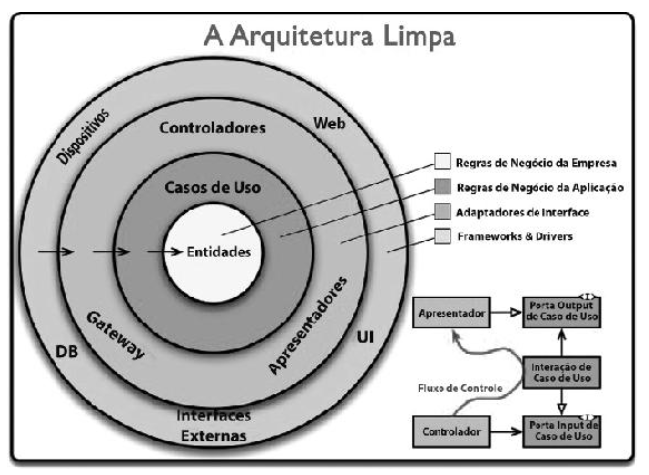
\includegraphics[width=0.6\textwidth]{imagens/ac_limpa_1.png}
    \fonte{Arquitetura Limpa (2017, Figura 22.1).}
\end{figure}

\subsection{Princípios SOLID}

A base para a criação de componentes de nível médio bem projetados, tolerantes a mudanças e fáceis de compreender é o conjunto de princípios SOLID \cite{martin2017}. Estes princípios orientam a organização de funções e estruturas de dados em classes e módulos isolados:

\begin{enumerate}[label=\alph*)]
    \item \textbf{SRP (Princípio da Responsabilidade Única)}: estabelece que um módulo deve ser responsável por um, e apenas um, ator;
    \item \textbf{OCP (Princípio Aberto/Fechado)}: um artefato de software deve ser aberto para extensão, mas fechado para modificação;
    \item \textbf{LSP (Princípio de Substituição de Liskov)}: para que sistemas sejam construídos a partir de partes intercambiáveis, essas partes devem aderir a um contrato que permita substituição sem alterar o funcionamento do programa;
    \item \textbf{ISP (Princípio da Segregação de Interface)}: orienta os projetistas a não dependerem de coisas que não utilizam;
    \item \textbf{DIP (Princípio da Inversão de Dependência)}: o código que implementa políticas de alto nível não deve depender de detalhes de baixo nível. As dependências de código-fonte devem referir-se apenas a abstrações.
\end{enumerate}

\subsection{Camadas do Projeto e Reprodutibilidade}

Neste projeto de análise de redes parlamentares, os princípios da Arquitetura Limpa e SOLID foram aplicados na definição da topologia dos diretórios. O código-fonte é estritamente isolado dos artefatos de dados gerados (\texttt{data/}), estruturando-se nas seguintes camadas modulares:

\begin{enumerate}[label=\alph*)]
    \item \textbf{Models}: representa a camada de Entidades, abrigando classes cruciais e independentes como \texttt{Deputy}, \texttt{Proposition} e a estrutura central da rede;
    \item \textbf{Core}: atua como a camada de Casos de Uso, orquestrando a lógica pesada de grafos e centralizando algoritmos matemáticos e de detecção de comunidades, isolados de preocupações de entrada e saída (I/O);
    \item \textbf{Extraction, Processing e Visualization}: atuam como Adaptadores de Interface, consumindo dados brutos do dataset da Câmara e processando visualizações gráficas de maneira desacoplada das regras de negócio;
    \item \textbf{Repository}: camada que abstrai os Drivers, responsável pela persistência do banco de dados local e exportação de artefatos (\texttt{.csv}, \texttt{.gexf} e \texttt{.json}).
\end{enumerate}

\section{TEORIA DOS GRAFOS E CIÊNCIA DE REDES}
A modelagem de sistemas complexos, como o ecossistema legislativo, exige uma base matemática rigorosa capaz de representar as interações entre os seus atores. Essa base é fornecida pela Teoria dos Grafos, que atua como o alicerce estrutural para a Ciência de Redes. Nas subseções seguintes, são definidos os conceitos topológicos, a modelagem de interações sociais e as métricas analíticas que viabilizam a extração de inteligência a partir de dados relacionais brutos \cite{newman2010, diestel2017}.
\subsection{Fundamentos de Redes Complexas e Grafos}

Na sua forma mais elementar, uma rede (ou grafo, na literatura matemática) é um catálogo dos componentes de um sistema e das interações diretas entre eles. Conforme \citeonline{barabasi2016} e \citeonline{diestel2017}, esses componentes são frequentemente chamados de nós (ou vértices) e as interações são chamadas de ligações (ou arestas), conforme a formulação matemática a seguir:

\begin{equation}
G = (V, E, w)
\end{equation}

Onde:
\begin{itemize}
    \item $V$ é o conjunto de vértices (nós);
    \item $E \subseteq V \times V$ é o conjunto de arestas;
    \item $w: E \to \mathbb{R}$ é a função de peso que associa um valor real a cada aresta.
\end{itemize}

A representação de um grafo visualmente:

\begin{figure}[H]
    \centering
    \caption{Representação de um grafo desconexo não direcionado.}
    \label{fig:grafo_1}
    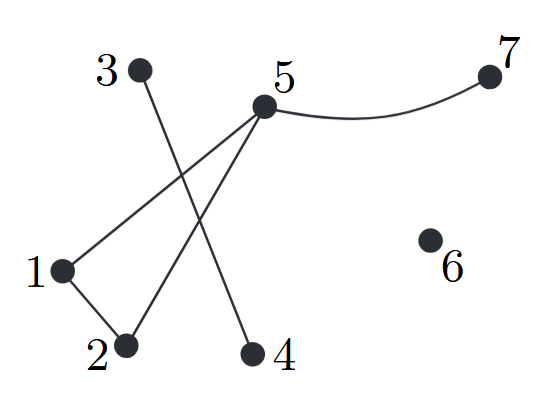
\includegraphics[width=0.6\textwidth]{imagens/grafo_1.png}
    \fonte{Diestel (2017, p. 2).}
\end{figure}

A topologia de uma rede é ditada pela natureza de suas arestas. Barabási explica que os grafos podem ser direcionados, quando a relação possui um sentido único (como um link na World Wide Web), ou não direcionados, quando a relação é mútua e de via dupla (como uma linha de transmissão de energia). Além da direção, as redes do mundo real frequentemente possuem conexões com intensidades diferentes. Para modelar essas intensidades, utilizam-se os grafos ponderados, onde cada aresta recebe um peso numérico.

Sob a ótica da Ciência da Computação, a eficiência no processamento dessas redes depende intrinsecamente de como o grafo é alocado na memória. \citeonline{cormen2009} detalha que existem dois modos padrões para a representação computacional: através de uma coleção de listas de adjacências ou através de uma matriz de adjacências. Enquanto a matriz consome um espaço de memória quadrático em relação aos vértices, a representação por lista de adjacências é o método preferido por oferecer uma estrutura muito mais compacta para grafos esparsos --- aqueles em que o número de arestas é muito menor que o máximo possível.

\subsection{Grafos Bipartidos e Projeção Unimodal}

Uma classe particular de grafos ocupa posição central na modelagem adotada neste trabalho: os grafos bipartidos. Um grafo é dito bipartido quando seu conjunto de vértices pode ser particionado em dois subconjuntos disjuntos $U$ e $V$, tais que $U \cap V = \emptyset$, de modo que toda aresta conecta necessariamente um vértice de $U$ a um vértice de $V$, nunca dois vértices pertencentes ao mesmo subconjunto \cite{diestel2017}. Na literatura de Ciência de Redes, essa estrutura é frequentemente denominada rede bimodal (\textit{two-mode network}) ou rede de afiliação (\textit{affiliation network}), sendo o exemplo canônico a relação entre um conjunto de pessoas e um conjunto de grupos ou eventos aos quais elas pertencem \cite{newman2010}, conforme o exemplo de um grafo bipartido abaixo:

\begin{figure}[H]
    \centering
    \caption{Representações de grafos bipartidos}
    \label{fig:grafo_bipartido}
    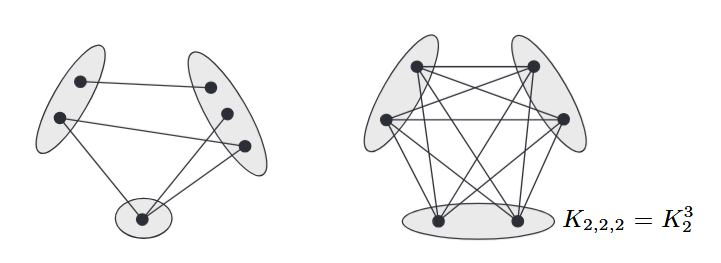
\includegraphics[width=0.6\textwidth]{imagens/graph_bipartid_1.png}
    \fonte{Diestel (2017, p. 15).}
\end{figure}

Como grafos bipartidos representam dois tipos distintos de entidade simultaneamente, sua análise direta por métricas de centralidade convencionais torna-se pouco intuitiva. A técnica usual consiste em derivar, a partir do grafo bipartido, uma rede unimodal (\textit{one-mode}) por meio de uma operação de \textbf{projeção}. Na projeção sobre o subconjunto $U$, dois vértices de $U$ passam a ser conectados sempre que compartilham ao menos um vizinho comum em $V$ \cite{newman2010}. Transpondo essa definição para o objeto deste trabalho, a projeção sobre o conjunto de deputados conecta dois parlamentares sempre que ambos assinam uma mesma proposição legislativa, produzindo a rede de coautoria efetivamente analisada.

A operação de projeção, contudo, introduz uma distorção estrutural conhecida. Cada elemento do subconjunto projetado que agrega $n$ vértices do outro lado gera, na projeção, um subgrafo completo (clique) de $\binom{n}{2}$ arestas. Em consequência, grupos numerosos --- proposições com muitos coautores, no caso legislativo --- produzem, sozinhos, um volume desproporcional de arestas, dominando a topologia resultante e suprimindo o sinal das colaborações menores e mais específicas. Esse fenômeno de inflação de arestas é precisamente a motivação teórica para a heurística de ponderação e para os filtros de massa de signatários formalizados no Capítulo~\ref{cap:metodologia}.

O tratamento clássico para essa distorção foi proposto por \citeonline{newman2001} no estudo de redes de colaboração científica, ao ponderar cada colaboração de forma inversamente proporcional ao número de coautores do trabalho compartilhado. A fórmula de ponderação adotada neste trabalho constitui uma adaptação direta desse princípio ao contexto parlamentar, cuja formalização completa --- incluindo os filtros qualitativos derivados --- é apresentada na Seção de modelagem do Capítulo~\ref{cap:metodologia}.

\subsection{Modelagem de Redes Sociais e Coautoria}

Ao aplicar a Teoria dos Grafos à sociologia, originam-se as chamadas redes sociais. Segundo \citeonline{newman2010}, nas redes sociais os vértices representam pessoas (ou grupos de pessoas), denominados atores, e as arestas representam alguma forma de interação social entre eles, comumente chamadas de laços (\textit{ties}), conforme a figura a seguir, que representa uma rede de atores de Hollywood, na qual dois atores estão conectados se atuaram no mesmo filme:
\begin{figure}[H]
    \centering
    \caption{Representação de um grafo aplicado ao contexto}
    \label{fig:hollywood}
    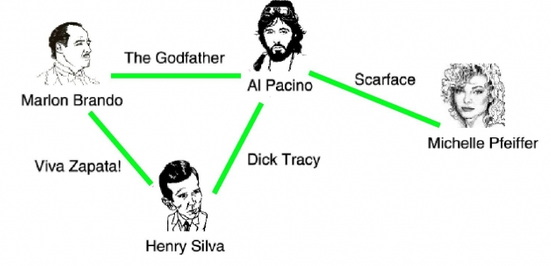
\includegraphics[width=0.6\textwidth]{imagens/barabasi_1.png}
    \fonte{Barabási (2016).}
\end{figure}

Uma classe especialmente útil de redes sociais abordada por Newman são as redes de avaliação, onde os atores são conectados através da participação conjunta em grupos ou eventos. Um exemplo clássico e direto dessa estrutura é a rede de coautoria. Na academia, por exemplo, um ator é um autor científico e o laço é formado quando dois autores assinam um mesmo artigo.

No contexto da Câmara dos Deputados abordado neste projeto, essa exata estrutura de coautoria é adotada para a modelagem do ecossistema legislativo: os parlamentares assumem o papel de vértices e as proposições legislativas (como Projetos de Lei e PECs) assinadas em conjunto formam as arestas ponderadas da rede. Através dessa modelagem, é possível transformar assinaturas em documentos sociais em um grafo tangível de articulação política.

\subsection{Métricas de Centralidade e Influência}
\label{subsec:metricas}

Com a topologia da rede computacionalmente definida, a Ciência de Redes atua quantificando a importância estrutural de cada vértice. \citeonline{newman2010} aponta que grande parte da pesquisa em redes busca responder à pergunta: quais são os vértices mais importantes ou centrais em uma rede? Para responder a isso, existem diversas métricas matemáticas que capturam diferentes perspectivas do que significa ter influência. Neste trabalho, destacam-se quatro métricas principais:

\begin{enumerate}[label=\alph*)]
    \item \textbf{Centralidade de Grau (\textit{Degree})}: é a medida mais intuitiva de centralidade, definida como o número de conexões diretas que um indivíduo possui. A premissa analítica é direta: atores com mais conexões diretas possuem maior acesso à informação e maior influência imediata no seu círculo. Em grafos ponderados (frequentemente denominada força ou \textit{strength} do nó), o grau é calculado como o somatório dos pesos das arestas incidentes naquele vértice:

    \begin{equation}
    s_i = \sum_{j \in N(i)} w(i,j)
    \label{eq:grau_ponderado}
    \end{equation}

    onde $s_i$ representa a soma dos pesos das arestas incidentes no vértice $i$, e $N(i)$ representa o conjunto de vizinhos diretos de $i$.

    \item \textbf{Centralidade de Intermediação (\textit{Betweenness})}: desenvolvida inicialmente pelo sociólogo Linton Freeman (\citeyear{freeman1977}), esta métrica avalia a frequência com que um vértice atua como uma ponte ao longo dos caminhos mínimos (geodésicos) entre outros pares de vértices na rede. Matematicamente, ela é a razão entre o número total de caminhos mínimos conectando dois nós e a quantidade absoluta desses caminhos que passam pelo vértice em questão:

    \begin{equation}
    C_B(v) = \sum_{s \neq v \neq t} \frac{\sigma_{st}(v)}{\sigma_{st}}
    \label{eq:betweenness}
    \end{equation}

    onde $C_B(v)$ é a fração de caminhos mínimos entre todos os pares que passam por $v$ \cite{freeman1977}.
    
    \item \textbf{Centralidade de Proximidade (\textit{Closeness})}: esta métrica avalia a distância geodésica média de um vértice em relação a todos os outros vértices acessíveis na rede. Nós com alta proximidade conseguem disseminar ideias ou influenciar toda a comunidade de maneira mais ágil:

    \begin{equation}
    C_C(v) = \frac{n-1}{\sum_{u \neq v} d(v,u)}
    \label{eq:closeness}
    \end{equation}

    onde $C_C(v)$ é o inverso da soma das distâncias geodésicas do vértice $v$ a todos os outros vértices da rede.
    
    \item \textbf{Centralidade de Autovetor (\textit{Eigenvector})}: uma extensão natural do grau, a centralidade de autovetor pondera a qualidade das relações \cite{bonacich1972}. O modelo matemático propõe que a importância de um vértice é proporcional à soma das importâncias dos seus vizinhos, incorporando o peso das conexões na versão ponderada:

    \begin{equation}
    C_E(v) = \frac{1}{\lambda} \sum_{u \in N(v)} w(v,u) C_E(u)
    \label{eq:eigenvector}
    \end{equation}

    em que $\lambda$ é o maior autovalor da matriz de adjacências ponderada da rede \cite{bonacich1987}.
\end{enumerate}

\section{DETECÇÃO DE COMUNIDADES (AGRUPAMENTOS PARLAMENTARES)}

A detecção de comunidades é o processo de encontrar divisões naturais em uma rede, buscando grupos de vértices onde existem muitas arestas internamente e poucas arestas conectando grupos distintos. Segundo \citeonline{newman2010}, diferentemente do particionamento de grafos tradicional (onde o número e o tamanho dos grupos são rigidamente predefinidos), a detecção de comunidades é uma ferramenta exploratória que busca descobrir a estrutura de larga escala de forma autônoma. No contexto deste projeto, as comunidades extraídas do grafo representam os agrupamentos parlamentares, revelando blocos partidários, facções informais ou fortes alinhamentos ideológicos no legislativo.

\subsection{Modularidade (Q)}

A modularidade é a métrica formal mais consolidada para avaliar a qualidade de uma partição em comunidades em uma rede. Proposta originalmente por \cite{newman2004} e formalizada matematicamente em \cite{newman2010}, a modularidade $Q$ mede a diferença entre a fração de arestas que conectam vértices da mesma comunidade no grafo observado e a fração esperada em um grafo aleatório com a mesma sequência de graus. Sua formulação matemática é:

\begin{equation}
    Q = \frac{1}{2m} \sum_{i,j} \left[ A_{ij} - \frac{k_i k_j}{2m} \right] \delta(c_i, c_j)
    \label{eq:modularidade}
\end{equation}

Onde $A_{ij}$ é a matriz de adjacências (igual ao peso da aresta $w_{ij}$ em grafos ponderados), $k_i$ é o grau do vértice $i$, $m$ é o número total de arestas, $c_i$ é a comunidade à qual o vértice $i$ pertence, e $\delta(c_i, c_j)$ é a função delta de Kronecker, igual a 1 se $c_i = c_j$ e 0 caso contrário.

Valores de $Q$ variam tipicamente entre $-0{,}5$ e $1$. Conforme \citeonline{newman2010}, valores acima de $0{,}3$ indicam estrutura comunitária significativa em redes reais; valores próximos de zero indicam que a partição é estatisticamente indistinguível da aleatória; e valores negativos indicam anti-comunidades. A modularidade fornece, portanto, um critério objetivo para comparar partições alternativas geradas por diferentes algoritmos.

Um aspecto central da formulação da modularidade merece destaque, pois fundamenta o procedimento de validação estatística adotado neste trabalho. O termo $k_i k_j / 2m$ presente na Equação~\ref{eq:modularidade} não é arbitrário: ele representa o peso ou intensidade esperada da conexão entre os vértices $i$ e $j$ em um \textbf{modelo nulo}, isto é, em um grafo aleatório que preserva a sequência de graus da rede original mas redistribui as conexões ao acaso \cite{newman2010}. A modularidade mede, portanto, exatamente o excesso de arestas internas às comunidades em relação ao que se esperaria por puro acaso, dada a mesma distribuição de graus.

Esse modelo nulo, conhecido na literatura como \textit{configuration model}, é a referência estatística contra a qual a significância de uma estrutura comunitária pode ser avaliada. Uma modularidade elevada só constitui evidência robusta de organização não-aleatória quando supera de forma clara os valores obtidos sobre realizações desse modelo nulo. É precisamente essa comparação --- entre a modularidade observada e a distribuição de modularidades de grafos nulos com igual sequência de graus --- que o Capítulo~\ref{cap:metodologia} formaliza como teste de permutação, e cujos resultados são reportados no Capítulo~\ref{cap:resultados}.

\subsection{Algoritmo de Louvain}

O algoritmo de Louvain, proposto por \cite{blondel2008}, é um método heurístico de otimização gulosa que busca maximizar a modularidade $Q$ por meio de duas fases iterativas. Na primeira fase, cada vértice é inicialmente atribuído à sua própria comunidade. Em seguida, para cada vértice $i$, considera-se a remoção de $i$ de sua comunidade atual e sua inserção em cada uma das comunidades de seus vizinhos, escolhendo o movimento que produz o maior ganho positivo em $Q$. A fase termina quando nenhum movimento produz ganho. Na segunda fase, as comunidades resultantes são contraídas em supernodos e o processo recomeça. As iterações continuam até que nenhuma mudança aumente a modularidade.

Sua popularidade decorre de três propriedades práticas: (i) complexidade computacional aproximadamente linear no número de arestas para grafos esparsos, viabilizando aplicação a redes com milhares de nós; (ii) qualidade comparável a algoritmos exatos em benchmarks como o de \cite{lancichinetti2008}; e (iii) implementações maduras na biblioteca NetworkX, garantindo reprodutibilidade.

Há, contudo, uma limitação conhecida: o algoritmo é sensível à ordem de processamento dos vértices, podendo produzir partições ligeiramente diferentes em execuções distintas. No presente trabalho, esse efeito foi controlado pela fixação de uma semente aleatória (\textit{seed}) constante.

No artigo original do Louvain, \citeonline{blondel2008} apresentam a fórmula exata usada na primeira fase do algoritmo. Ela calcula, com baixíssimo custo computacional, qual seria a variação de modularidade ($\Delta Q$), ou ganho de modularidade, ao mover um nó isolado $i$ para dentro de uma comunidade vizinha $C$:

\begin{equation}
\Delta Q = \left[ \frac{\Sigma_{in} + 2k_{i,in}}{2m} - \left( \frac{\Sigma_{tot} + k_i}{2m} \right)^2 \right] - \left[ \frac{\Sigma_{in}}{2m} - \left( \frac{\Sigma_{tot}}{2m} \right)^2 - \left( \frac{k_i}{2m} \right)^2 \right]
\label{eq:delta_q}
\end{equation}

onde $\Sigma_{in}$ é a soma dos pesos das arestas internas à comunidade $C$, $\Sigma_{tot}$ é a soma dos pesos de todas as arestas incidentes em vértices de $C$, $k_i$ é o grau ponderado do vértice $i$, $k_{i,in}$ é a soma dos pesos das arestas de $i$ para vértices já pertencentes a $C$, e $m$ é a soma dos pesos de todas as arestas da rede.

No livro \textit{Networks}, \citeonline{newman2010} demonstra que, para fins de particionamento de grafos e otimização espectral, a modularidade pode ser reescrita elegantemente em notação matricial:

\begin{equation}
Q = \frac{1}{2m}\, \mathbf{s}^{\top} \mathbf{B}\, \mathbf{s}
\label{eq:mod_matricial}
\end{equation}

onde $\mathbf{s}$ é o vetor de atribuição de comunidades e $\mathbf{B}$ é a chamada matriz de modularidade, definida por $B_{ij} = A_{ij} - k_i k_j / 2m$.

\subsection{Algoritmo Label Propagation}

O algoritmo Label Propagation, proposto por \citeonline{raghavan2007}, parte de uma abordagem distinta: em vez de otimizar uma função objetivo global, ele propaga rótulos locais entre vértices vizinhos até a convergência por meio de um processo de busca por consenso. Inicialmente, cada vértice recebe um rótulo único. Na formulação clássica síncrona do algoritmo, o rótulo de um nó $x$ no passo iterativo $t$ é determinado estritamente a partir dos rótulos de seus vizinhos no passo anterior $t-1$, conforme a Equação~\ref{eq:lpa_sincrono}:

\begin{equation}
C_x(t) = f\left( C_{x_1}(t-1), C_{x_2}(t-1), \dots, C_{x_k}(t-1) \right)
\label{eq:lpa_sincrono}
\end{equation}

onde $x_1, \dots, x_k$ são os vizinhos diretos de $x$ e a função $f$ retorna o rótulo de maior frequência (moda) entre os vizinhos, resolvendo empates de forma uniformemente aleatória. No entanto, estruturas bipartidas ou em formato de estrela causam oscilações infinitas de rótulos sob essa dinâmica síncrona. Para contornar essa limitação estrutural, os autores propõem uma dinâmica de atualização assíncrona, expressa na Equação~\ref{eq:lpa_assincrono}:

\begin{equation}
C_x(t) = f\left( C_{x_{i_1}}(t), \dots, C_{x_{i_m}}(t), C_{x_{i_{m+1}}}(t-1), \dots, C_{x_{i_k}}(t-1) \right)
\label{eq:lpa_assincrono}
\end{equation}

onde os vizinhos indexados de $i_1$ a $i_m$ já foram atualizados no passo corrente $t$, enquanto os vizinhos de $i_{m+1}$ a $i_k$ mantêm os rótulos do passo anterior $t-1$. 

Seja $d_i^{C_j}$ a soma dos pesos das arestas do nó $i$ conectadas a vizinhos com o rótulo $C_j$. O processo iterativo de propagação assíncrona encerra-se estritamente quando, para cada nó $i$ que carrega um rótulo $C_m$, a Equação~\ref{eq:lpa_criterio_parada} é satisfeita para todos os rótulos alternativos $j$ ativos na rede:

\begin{equation}
d_i^{C_m} \ge d_i^{C_j}, \quad \forall j
\label{eq:lpa_criterio_parada}
\end{equation}

Isso garante estabilidade local, uma vez que nenhum vértice individualmente terá incentivo para alterar seu agrupamento comunitário.

\section{TRABALHOS CORRELATOS}

A aplicação de análise de redes ao comportamento legislativo não é inédita, e situar o presente trabalho nesse cenário é essencial para delimitar sua contribuição. Esta seção revisa, de forma sintética, os principais antecedentes internacionais e nacionais que orientam a modelagem aqui adotada.

No cenário internacional, o marco fundador da análise de redes de coautoria legislativa é o trabalho de \citeonline{fowler2006}, que modelou a rede de coautoria (\textit{cosponsorship}) do Congresso dos Estados Unidos e demonstrou que a posição estrutural de um parlamentar na rede --- e não apenas sua filiação partidária --- é preditora de influência legislativa. Esse estudo estabeleceu a coautoria como \textit{proxy} mensurável de articulação política e consolidou o uso de métricas de centralidade como indicadores de poder informal, abordagem diretamente adotada neste trabalho.

No cenário brasileiro, a literatura sobre comportamento legislativo tradicionalmente privilegia a análise de votações nominais como indicador de coesão e disciplina partidária. \citeonline{figueiredo1998} constituem referência central ao evidenciar que o presidencialismo de coalizão brasileiro produz padrões de comportamento agregado por blocos, enquanto \citeonline{zucco2009} discute a heterogeneidade interna dos partidos e os limites da filiação como preditor de alinhamento. Este trabalho dialoga com essa tradição, mas dela se distingue ao adotar a coautoria --- e não a votação --- como substrato relacional, e ao priorizar a construção de um artefato de software reprodutível.

É justamente nesse cruzamento que reside a lacuna endereçada: são raros, no contexto brasileiro, os estudos que combinam análise formal de redes de coautoria, cobertura multi-anual recente e disponibilização de código-fonte auditável. O presente trabalho posiciona-se nessa interseção, aproximando o instrumental consolidado por \cite{fowler2006} da realidade da Câmara dos Deputados do Brasil, com ênfase em reprodutibilidade computacional.

%-------------------------------------------------------------------------------------%
\chapter{Metodologia}
\label{cap:metodologia}

Este capítulo descreve o paradigma de pesquisa adotado, os procedimentos de coleta e
tratamento dos dados, a estratégia de modelagem do grafo parlamentar, a seleção dos algoritmos
e métricas analíticas, a medida de robustez das partições e os procedimentos de
validação aplicados ao artefato construído.

\section{CARACTERIZAÇÃO DA PESQUISA}

A natureza desta pesquisa é caracterizada como aplicada, com abordagem quantitativa e finalidade exploratório-descritiva. Aplicada, pois objetiva a construção de um artefato de software com propósito prático imediato. Quantitativa, pois fundamenta-se em métricas matematicamente formalizadas e em teste estatístico de significância. Exploratório-descritiva, pois pretende não apenas descrever a estrutura da rede legislativa, mas também explorar relações que ainda não foram sistematicamente quantificadas para o período 2022--2025.

\subsection{O Método DSR (Design Science Research)}

O paradigma metodológico adotado neste trabalho é o \textit{Design Science Research} (DSR), conforme formalizado por \citeonline{hevner2004} e \citeonline{wieringa2014}. Diferentemente das ciências naturais, que explicam fenômenos existentes, e das ciências sociais empíricas, que descrevem comportamentos observáveis, o DSR é orientado à \textbf{produção de artefatos} (constructos, modelos, métodos ou instanciações de software) projetados para solucionar problemas práticos identificados em um contexto real \cite{hevner2004, wieringa2014}.

Como ilustrado no framework clássico de \citeonline{hevner2004} (~\ref{fig:dsr_framework}), a condução desta pesquisa estabelece uma sinergia rigorosa entre três domínios fundamentais:
\begin{itemize}
    \item O \textbf{Ambiente} prático da Câmara dos Deputados, que define as necessidades analíticas e fornece os dados brutos de proposições e coautorias;
    \item A \textbf{Base de Conhecimento} científico, que fornece as fundações teóricas (ciência de redes e teoria dos grafos) e as metodologias de desenvolvimento (princípios arquiteturais de software e testes);
    \item O \textbf{Espaço de Pesquisa} em si, focado na construção (implementação do pipeline analítico em Python) e na avaliação iterativa do artefato gerado.
\end{itemize}

\begin{figure}[H]
    \centering
    \caption{Framework de Pesquisa em Design Science}
    \label{fig:dsr_framework}
    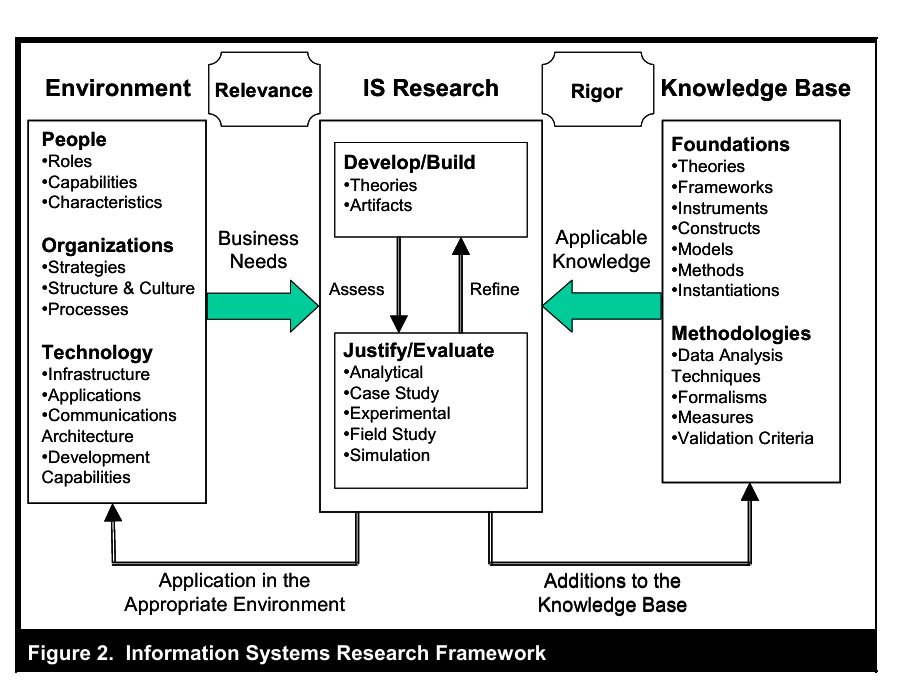
\includegraphics[width=0.75\textwidth]{imagens/hevner_DSR_1.png}
    \fonte{Adaptado de Hevner et al. \cite[p. 80]{hevner2004}.}
\end{figure}

Para orquestrar essas frentes, a investigação estrutura-se em torno de três ciclos dinâmicos propostos na literatura de DSR \cite{hevner2004}: o \textit{ciclo de relevância}, que conecta o ambiente do problema às exigências do artefato; o \textit{ciclo de rigor}, que fundamenta o desenvolvimento na base de conhecimento existente; e o \textit{ciclo de design} propriamente dito, que executa iterativamente as fases de construção e avaliação até que o artefato atinja a maturidade necessária para responder ao problema analítico mapeado.

\subsection{Fases do Método}

O ciclo DSR foi instanciado neste trabalho nas seguintes fases:

\begin{enumerate}[label=\alph*)]
    \item \textbf{Identificação do problema}: constatação da lacuna entre a abundância de dados legislativos abertos da Câmara dos Deputados e a escassez de ferramentas analíticas reprodutíveis capazes de extrair, desses dados, evidências mensuráveis sobre estruturas de influência política;

    \item \textbf{Definição de objetivos}: estabelecimento dos requisitos do artefato --- modularidade, reprodutibilidade, cobertura por testes, interoperabilidade com ferramentas externas (Gephi) e independência da fonte de dados;

    \item \textbf{Projeto e desenvolvimento}: construção iterativa do software seguindo Arquitetura Limpa \cite{martin2017} e princípios SOLID, com cobertura por testes automatizados desde o início (TDD parcial);

    \item \textbf{Demonstração}: execução do pipeline completo para os anos 2022, 2023, 2024 e 2025, gerando os artefatos de dados (CSV, GEXF, SQLite e JSON);

    \item \textbf{Avaliação}: validação técnica (suíte de testes) e validação científica (teste de permutação contra modelo nulo);

    \item \textbf{Comunicação}: disponibilização do código-fonte em repositório aberto, documentação técnica e elaboração do presente trabalho.
\end{enumerate}

\subsection{Uso de Ferramentas de Inteligência Artificial}

Em conformidade com as orientações de integridade acadêmica, registra-se que ferramentas de inteligência artificial generativa, baseadas em modelos de linguagem, foram utilizadas de forma auxiliar durante a elaboração deste trabalho. Seu uso restringiu-se a: apoio à revisão gramatical e à clareza da redação; sugestão de estruturas e organização textual; e auxílio à compreensão e discussão de conceitos técnicos. A concepção do artefato, as decisões de projeto e de modelagem, a implementação do código, a interpretação dos resultados e a autoria intelectual do trabalho são de responsabilidade exclusiva do autor.

\section{PROCEDIMENTOS DE COLETA E TRATAMENTO DE DADOS}
\label{sec:procedimentos}

Para subsidiar a modelagem da rede parlamentar e viabilizar o cálculo de centralidades e a identificação de comunidades, estruturou-se um pipeline sistemático de aquisição e processamento de dados. Esse fluxo operacional compreende etapas sequenciais que vão desde o consumo automatizado das bases públicas oficiais até a persistência das redes resultantes em formatos padronizados de alta interoperabilidade. Em conformidade com as diretrizes de desacoplamento da Arquitetura Limpa, todo o fluxo de ingestão e higienização de dados é tratado de maneira isolada do núcleo analítico da aplicação. Essa separação física e lógica entre as rotinas de extração (\textit{I/O}) e as regras de negócio assegura a integridade das métricas calculadas e garante a reprodutibilidade estrita do pipeline para toda a série temporal analisada, compreendida entre os anos de 2022 e 2025.

\subsection{Fonte dos Dados}

A fonte primária de dados é o Portal de Dados Abertos da Câmara dos Deputados (\url{https://dadosabertos.camara.leg.br}), mantido pela própria instituição em cumprimento à Lei de Acesso à Informação (Lei 12.527/2011). Trata-se da \textbf{fonte oficial primária} dos registros legislativos brasileiros, sem autoridade superior de referência. Eventuais inconsistências da fonte representam limitação intrínseca ao registro público nacional e estão fora do escopo deste trabalho.

Foram utilizados dois conjuntos de arquivos CSV por ano analisado:

\begin{itemize}
    \item \texttt{proposicoesAutores-YYYY.csv}: contém o vínculo entre cada proposição e seus respectivos autores, fornecendo o substrato relacional para construção das arestas;
    \item \texttt{proposicoes-YYYY.csv}: contém os metadados de cada proposição, incluindo o tipo (PL, PEC, PLP etc.), utilizado para aplicação dos filtros de relevância.
\end{itemize}

O download foi automatizado com cache local: arquivos baixados em uma execução são reaproveitados em execuções subsequentes, garantindo reprodutibilidade exata mesmo diante de eventuais atualizações nos arquivos do portal.

\subsection{Recorte Temporal}

A delimitação do período em 2022--2025 resulta de critérios técnicos, e não de conveniência. Primeiro, \textbf{estabilidade e homogeneidade do esquema de dados}: os arquivos CSV anuais do Portal de Dados Abertos mantêm formato e cobertura consistentes no período recente, evitando a heterogeneidade de esquema e a degradação de completude observadas em séries mais antigas. Segundo, \textbf{coerência institucional}: o intervalo abrange uma legislatura completa (a 57\textsuperscript{a}, iniciada em 2023) somada ao ano de transição (2022, encerramento da 56\textsuperscript{a}), permitindo testar a \textit{persistência} da estrutura sob um regime legislativo estável, sem o confundimento de múltiplas mudanças de regras eleitorais e de composição partidária que um intervalo mais amplo (por exemplo, 2010--2025) introduziria. Terceiro, \textbf{viabilidade computacional e de auditoria}: quatro \textit{snapshots} anuais completos são suficientes para avaliar a estabilidade do padrão estrutural (H1) mantendo cada grafo integralmente reproduzível e inspecionável. A ampliação da série temporal é registrada como trabalho futuro.



\subsection{Ferramental de Processamento}

O ecossistema técnico utilizado é integralmente baseado em software livre:

\begin{itemize}
    \item \textbf{Python 3.11}: linguagem principal;
    \item \textbf{NetworkX 3.2} \cite{networkx}: representação, algoritmos de grafos e detecção de comunidades (Louvain e Label Propagation nativos);
    \item \textbf{pandas 2.2}: manipulação tabular e leitura dos CSVs;
    \item \textbf{pydantic} e \textbf{pydantic-settings}: configuração tipada e validada a partir do arquivo \texttt{.env};
    \item \textbf{matplotlib} e \textbf{seaborn}: visualização e geração de figuras;
    \item \textbf{pytest} com \textbf{pytest-cov}: validação automatizada e medição de cobertura;
    \item \textbf{Docker} e \textbf{Docker Compose}: empacotamento reprodutível do ambiente de execução.
\end{itemize}

\section{ESTRATÉGIA DE MODELAGEM E MITIGAÇÃO DE VIÉS}

Esta seção formaliza a transformação dos dados legislativos brutos em um objeto
matemático analisável e explicita as decisões tomadas para evitar que artefatos
do próprio processo de modelagem sejam confundidos com estrutura política real.
Primeiro define-se a topologia adotada --- o grafo bipartido de autoria e sua
projeção unimodal sobre o conjunto de deputados. Em seguida, trata-se do problema
central dessa projeção, a inflação de arestas, por meio de uma heurística de
ponderação e de filtros qualitativos sobre as proposições consideradas.

\subsection{Definição Topológica}
\label{subsec:def_topologica}


O ecossistema legislativo da Câmara dos Deputados forma naturalmente um \textbf{grafo bipartido} (ou rede de dois modos) $B = (V_B, E_B)$ \cite{barabasi2016, newman2010}, onde o conjunto de vértices é particionado em dois subconjuntos disjuntos, $V_B = D \cup P$ com $D \cap P = \emptyset$ \cite{diestel2017}:

\begin{itemize}
    \item $D$ é o conjunto de deputados federais ativos no período analisado;
    \item $P$ é o conjunto de proposições legislativas apresentadas no respectivo ano;
    \item $E_B$ é o conjunto de arestas de autoria, em que uma aresta não-direcionada existe entre um deputado $d \in D$ e uma proposição $p \in P$ se e somente se o deputado $d$ for autor ou coautor da proposição $p$ \cite{diestel2017}.
\end{itemize}

\begin{figure}[H]
    \centering
    \caption{Grafo bipartido de coautoria: deputados ($D$) e proposições ($P$),
    com $n_p$ indicando o número de coautores de cada matéria.}
    \label{fig:bipartid_coautoria}
    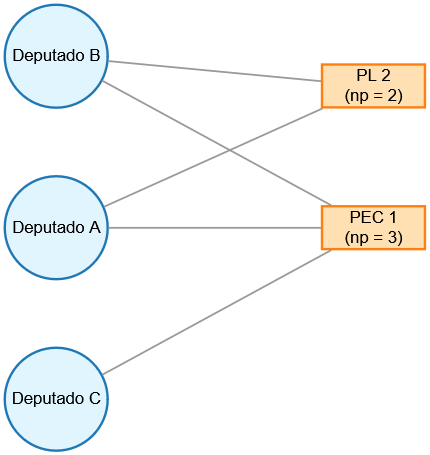
\includegraphics[width=0.55\textwidth]{imagens/bipartid_coautorias_1.png}
    \fonte{Elaborado pelo autor usando Graphviz Online (2026).}
\end{figure}

Esse grafo bipartido é transformado, por meio de uma \textbf{projeção unimodal} (ou de modo único) sobre o conjunto de deputados $D$, em uma rede de coautoria unimodal $G = (D, E', w)$ \cite{newman2010, barabasi2016}. Nessa projeção, dois deputados $i, j \in D$ são conectados por uma aresta em $E'$ se e somente se ambos assinarem pelo menos uma proposição em comum ($p \in P$), e o peso da aresta $w(i,j)$ codifica a intensidade dessa colaboração legislativa com base na relevância das matérias compartilhadas.

\begin{figure}[H]
    \centering
    \caption{Projeção unimodal do grafo bipartido da Figura~\ref{fig:bipartid_coautoria}
     sobre o conjunto $D$, com os pesos calculados pela
     Equação~\ref{eq:peso_coautoria}.}
    \label{fig:bipartid_projecao_unimodal}
    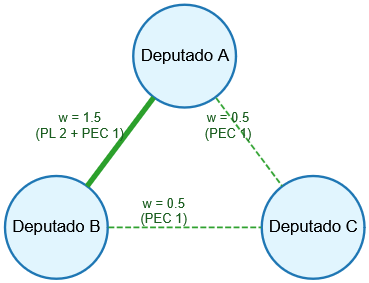
\includegraphics[width=0.5\textwidth]{imagens/unimodal_1.png}
    \fonte{Elaborado pelo autor usando Graphviz Online (2026).}
\end{figure}

A ~\ref{fig:bipartid_projecao_unimodal} materializa essa operação sobre o
exemplo da ~\ref{fig:bipartid_coautoria}. Como os deputados A e B assinam
em conjunto tanto o PL 2 ($n_p = 2$) quanto a PEC 1 ($n_p = 3$), a aresta que os
conecta acumula as duas contribuições. Já os pares A--C e B--C compartilham
apenas a PEC 1, recebendo uma única contribuição atenuada pelo número de
signatários. O deputado C, ausente do PL 2, não estabelece com A e B a mesma
intensidade de vínculo. A formalização do peso $w(i,j)$ que produz esses valores
é apresentada na subseção seguinte.

\subsection{Heurística de Ponderação e Normalização do Grafo}
\label{subsec:heuristica}

A definição do peso $w(i,j)$ das arestas na projeção unimodal é uma decisão metodológica crítica deste trabalho. Uma soma ingênua do número de coautorias simples mostra-se inadequada para o contexto legislativo: uma única Proposta de Emenda à Constituição (PEC), que frequentemente conta com mais de 200 signatários para atingir o quórum de apresentação, geraria, sozinha, um clique completo de $\binom{200}{2} = 19.900$ arestas com peso 1, distorcendo e dominando toda a estrutura topológica subsequente. 

Para mitigar esse viés de escala e capturar a verdadeira intensidade da colaboração política, adota-se a metodologia de projeção ponderada proposta por \citeonline{newman2010}:

\begin{equation}
w(i,j) = \sum_{p \in P_{ij}} \frac{1}{n_p - 1}
\label{eq:peso_coautoria}
\end{equation}

onde $P_{ij}$ representa o conjunto de proposições legislativas assinadas em comum por ambos os deputados $i$ e $j$, e $n_p$ é o número total de autores da proposição $p$, com a restrição de que $n_p \ge 2$ para todas as matérias em $P_{ij}$ (uma vez que coautorias exigem múltiplos autores). Sob essa formulação, a contribuição individual de cada proposição para a força da conexão decresce de forma inversamente proporcional ao seu número de signatários. Isso permite equilibrar a influência de coautorias em pequenos grupos (que possuem alta especificidade e indicam forte articulação política) e em grandes blocos de assinaturas (que possuem baixa especificidade analítica).

\begin{figure}[H]
    \centering
    \caption{Efeito da heurística de ponderação na projeção unimodal.}
    \label{fig:bipartid_projecao_unimodal2}
    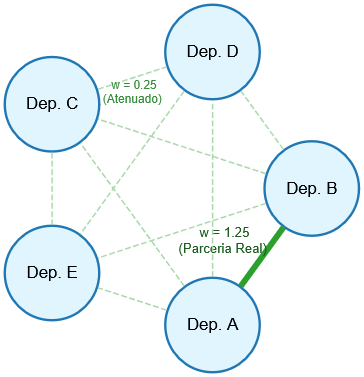
\includegraphics[width=0.5\textwidth]{imagens/unimodal_2.png}
    \fonte{Elaborado pelo autor usando Graphviz Online (2026).}
\end{figure}

A ~\ref{fig:bipartid_projecao_unimodal2} ilustra o efeito prático da
Equação~\ref{eq:peso_coautoria}. Considere uma PEC assinada pelos cinco
deputados do exemplo ($n_p = 5$) e um Projeto de Lei assinado exclusivamente
por A e B ($n_p = 2$). A PEC de massa conecta todos os $\binom{5}{2} = 10$
pares, mas com peso atenuado de $1/(5-1) = 0{,}25$ cada; o PL específico
acrescenta $1/(2-1) = 1{,}00$ apenas ao par A--B. O resultado é que a
articulação política efetiva entre A e B ($w = 1{,}25$) destaca-se em cinco
vezes sobre as conexões geradas pela assinatura coletiva ($w = 0{,}25$) ---
precisamente o comportamento que a heurística busca produzir.

Adicionalmente, três decisões qualitativas complementam a heurística:

\begin{enumerate}[label=\alph*)]
    \item \textbf{Filtro de tipos de proposição}: 
    Apenas proposições com conteúdo legislativo substantivo são consideradas: Projetos de Lei (PL), Propostas de Emenda à Constituição (PEC), Projetos de Lei Complementar (PLP), Projetos de Decreto Legislativo (PDL) e Emendas (EMC). Requerimentos, ofícios e proposições administrativas são excluídos.
    
    \item \textbf{Filtro de massa de signatários}: Proposições com mais de 30 deputados coautores são excluídas da construção de arestas. Empiricamente, a inclusão dessas matérias --- a maior delas uma PEC com 226 signatários --- eleva a densidade da rede de 9{,}9\% para 85{,}4\% em 2025, transformando-a em um grafo quase-completo e inviabilizando a detecção de comunidades (demonstração no Capítulo~\ref{cap:resultados}). Como consequência direta, \textbf{nenhuma PEC integra a rede de coautoria analisada}, pois todas superam o limiar de 30 --- resultado intencional, e não uma perda: a co-assinatura em massa reflete adesão agregada, não articulação coordenada, e sua exclusão é coerente com a definição de influência adotada. Cabe notar que a heurística de ponderação $1/(n_p-1)$ e este filtro são \textbf{complementares}: a primeira trata a distorção de \emph{peso} (cada par de uma PEC de massa contribui apenas $1/225$), enquanto o filtro trata a distorção \emph{topológica} --- a mera \emph{existência} das $\binom{226}{2} \approx 25\,\text{mil}$ arestas, que as métricas topológicas (intermediação, proximidade) e a própria densidade não conseguem ignorar. O limite de 30 é uma decisão conservadora, declarada como parâmetro sensível para análise de sensibilidade em trabalhos futuros.

    \item \textbf{Pesos uniformes por tipo de proposição}: Embora alguns trabalhos anteriores tenham experimentado pesos diferenciados por tipo (por exemplo, PEC com peso maior que PL), não existe na literatura uma escala teoricamente justificada para tal ponderação. Adota-se, portanto, peso igual a 1 para todos os tipos, sendo a seleção qualitativa realizada pelo filtro de tipos descrito acima.
\end{enumerate}

\section{SELEÇÃO DE ALGORITMOS E MÉTRICAS ANALÍTICAS}

A seleção das ferramentas analíticas orienta-se por dois critérios: consolidação
na literatura e disponibilidade de implementações maduras e auditáveis, requisito
derivado do compromisso de reprodutibilidade deste trabalho. As subseções a
seguir tratam, respectivamente, das métricas de centralidade adotadas e dos
algoritmos de detecção de comunidades.

\subsection{Métricas de Centralidade}

Quatro métricas de centralidade são computadas para cada deputado em cada ano, conforme definições formais apresentadas na Seção~\ref{subsec:metricas}.

Antes de aplicar essas métricas, é necessário entender o que se entende por influência neste trabalho. \textbf{Influência política é aqui operacionalizada, em sentido estritamente estrutural, como a posição de um deputado na rede de coautoria} --- e não como poder institucional formal (relatorias, presidência de comissões, controle de pauta), que se exerce por mecanismos não capturados pela coautoria. Especificamente, a influência estrutural é mensurada por duas dimensões complementares: a intermediação (\textit{betweenness}), que capta o papel de ponte entre grupos, na tradição de \cite{freeman1977}; e a centralidade de autovetor, que capta a inserção em vizinhanças bem conectadas \cite{bonacich1972}. Trata-se, portanto, de uma medida de articulação e colaboração legislativa, não de poder decisório --- distinção retomada na discussão dos resultados.

Dessa forma, cada métrica captura uma dimensão distinta de influência: grau pondera quantidade de colaborações; intermediação captura papel de ponte entre blocos; proximidade mede capacidade de disseminação; autovetor pondera a qualidade das conexões. Estas métricas compõem a caracterização descritiva das estruturas de influência da rede, apresentada no Capítulo~\ref{cap:resultados}.

Cada métrica emprega, ademais, a representação coerente com sua semântica. Grau e autovetor são calculados sobre o grafo \textbf{ponderado}, pois a intensidade da colaboração (afinidade) acumula-se de forma aditiva. Já intermediação e proximidade são calculadas sobre a topologia \textbf{não-ponderada}: em grafos ponderados, o peso é interpretado como distância ou custo, ao passo que na rede de coautoria o peso representa afinidade --- semântica inversa, cuja conciliação exigiria uma transformação arbitrária $1/w$. A intermediação é \textbf{normalizada} pelo fator $(n-1)(n-2)/2$ (grafos não-direcionados), produzindo valores em $[0,1]$ comparáveis entre anos de tamanhos distintos, requisito da análise temporal (Seção~\ref{sec:temporal}).

\subsection{Detecção de Comunidades}

Dois algoritmos são aplicados em paralelo:

\begin{enumerate}[label=\alph*)]
    \item \textbf{Louvain} \cite{blondel2008}: otimização gulosa da modularidade, executado com semente fixa (\textit{seed} $=$ 42) para garantir reprodutibilidade;
    \item \textbf{Label Propagation} \cite{raghavan2007}: propagação local de rótulos, utilizado como contraprova.
\end{enumerate}

O Louvain é considerado o método primário; o Label Propagation funciona como verificação de robustez --- quando ambos identificam estruturas similares, há maior confiança no achado.

\section{MEDIDA DE ROBUSTEZ: ADJUSTED RAND INDEX (ARI)}
\label{sec:ari}

Para avaliar a robustez da detecção de comunidades --- e, por consequência, a
solidez da hipótese central, compara-se a partição obtida pelo Louvain com a
obtida pelo Label Propagation por meio do \textit{Adjusted Rand Index} (ARI) \cite{hubert1985}. O
ARI mede a similaridade entre duas partições de um mesmo conjunto de nós,
corrigida para a concordância esperada ao acaso: o valor $1$ indica partições
idênticas (a menos de relabelagem), $0$ indica concordância ao nível do acaso e
valores negativos indicam concordância inferior à aleatória. O índice é computado
a partir da tabela de contingência entre as duas partições, e um ARI elevado é
interpretado como evidência de que a estrutura comunitária detectada é robusta à
escolha do algoritmo.

\section{AVALIAÇÃO DO ARTEFATO (PROCEDIMENTOS DE VALIDAÇÃO)}

A avaliação do artefato ocorre em duas frentes complementares, alinhadas à fase
de avaliação do ciclo DSR. A validação qualitativa confronta os achados com a
literatura sobre comportamento legislativo brasileiro; a quantitativa combina
teste estatístico de significância, cobertura por testes automatizados e
reprodutibilidade do ambiente de execução.

\subsection{Validação Qualitativa}

A validação qualitativa é realizada por meio da inspeção dos resultados frente à literatura política e ao conhecimento institucional sobre a Câmara dos Deputados. Especificamente, a hipótese detalhada no Capítulo~\ref{cap:introducao} é confrontada com os achados empíricos.

\subsection{Validação Quantitativa e Reprodutibilidade}

A validação quantitativa é executada em três níveis:

\begin{enumerate}[label=\alph*)]
    \item \textbf{Teste de permutação contra modelo nulo}: 
    Para verificar se a modularidade $Q_{\text{obs}}$ observada é estatisticamente significativa, são gerados 200 grafos aleatórios por meio do procedimento \textit{double-edge-swap}, que preserva exatamente a sequência de graus do grafo original mas randomiza a topologia. Como o \textit{double-edge-swap} redistribui as arestas sem seus pesos, o conjunto (\textit{multiset}) de pesos originais é reatribuído às arestas reconfiguradas, preservando a distribuição de pesos da rede real e assegurando que a comparação seja ponderada e homogênea com $Q_{\text{obs}}$. O $p$-value é estimado pelo estimador aditivo $p = (r+1)/(m+1)$, em que $r$ é o número de grafos nulos com $Q_{\text{nulo}} \geq Q_{\text{obs}}$ e $m$ é o número de permutações --- evitando que seja exatamente nulo, o que seria estatisticamente inválido em uma amostra finita. Adota-se nível de significância $\alpha = 0{,}05$.
    
    \item \textbf{Suíte de testes automatizados}:
    O artefato de software é validado por 210 testes automatizados (cobertura total 83\%, núcleo analítico $\geq$ 93\%), incluindo: (i) testes unitários sobre entidades de domínio e algoritmos; (ii) testes de integração sobre o pipeline; (iii) testes de integridade sobre os datasets gerados, parametrizados por ano (verificação de esquema, faixas de valores plausíveis, coerência CSV $\leftrightarrow$ GEXF).

    \item \textbf{Reprodutibilidade containerizada}:
    O ambiente de execução completo é encapsulado em imagem Docker, permitindo replicação exata em qualquer máquina com Docker instalado, independente de sistema operacional ou versões locais de bibliotecas.
\end{enumerate}

%-------------------------------------------------------------------------------------%
\chapter{Desenvolvimento}
\label{cap:desenvolvimento}

Este capítulo descreve a instanciação concreta do artefato de software --- denominado 
\textit{pipeline} --- conforme os princípios arquiteturais e a metodologia descritos nos capítulos anteriores.

\section{DEFINIÇÃO DA ARQUITETURA DO SISTEMA E ESTRUTURA MODULAR}

O pipeline é organizado em camadas com responsabilidades únicas, conforme o esquema:

\begin{figure}[H]
    \centering
    \caption{Diagrama de componentes e fluxo de dados do pipeline.}
    \label{fig:componentes}
    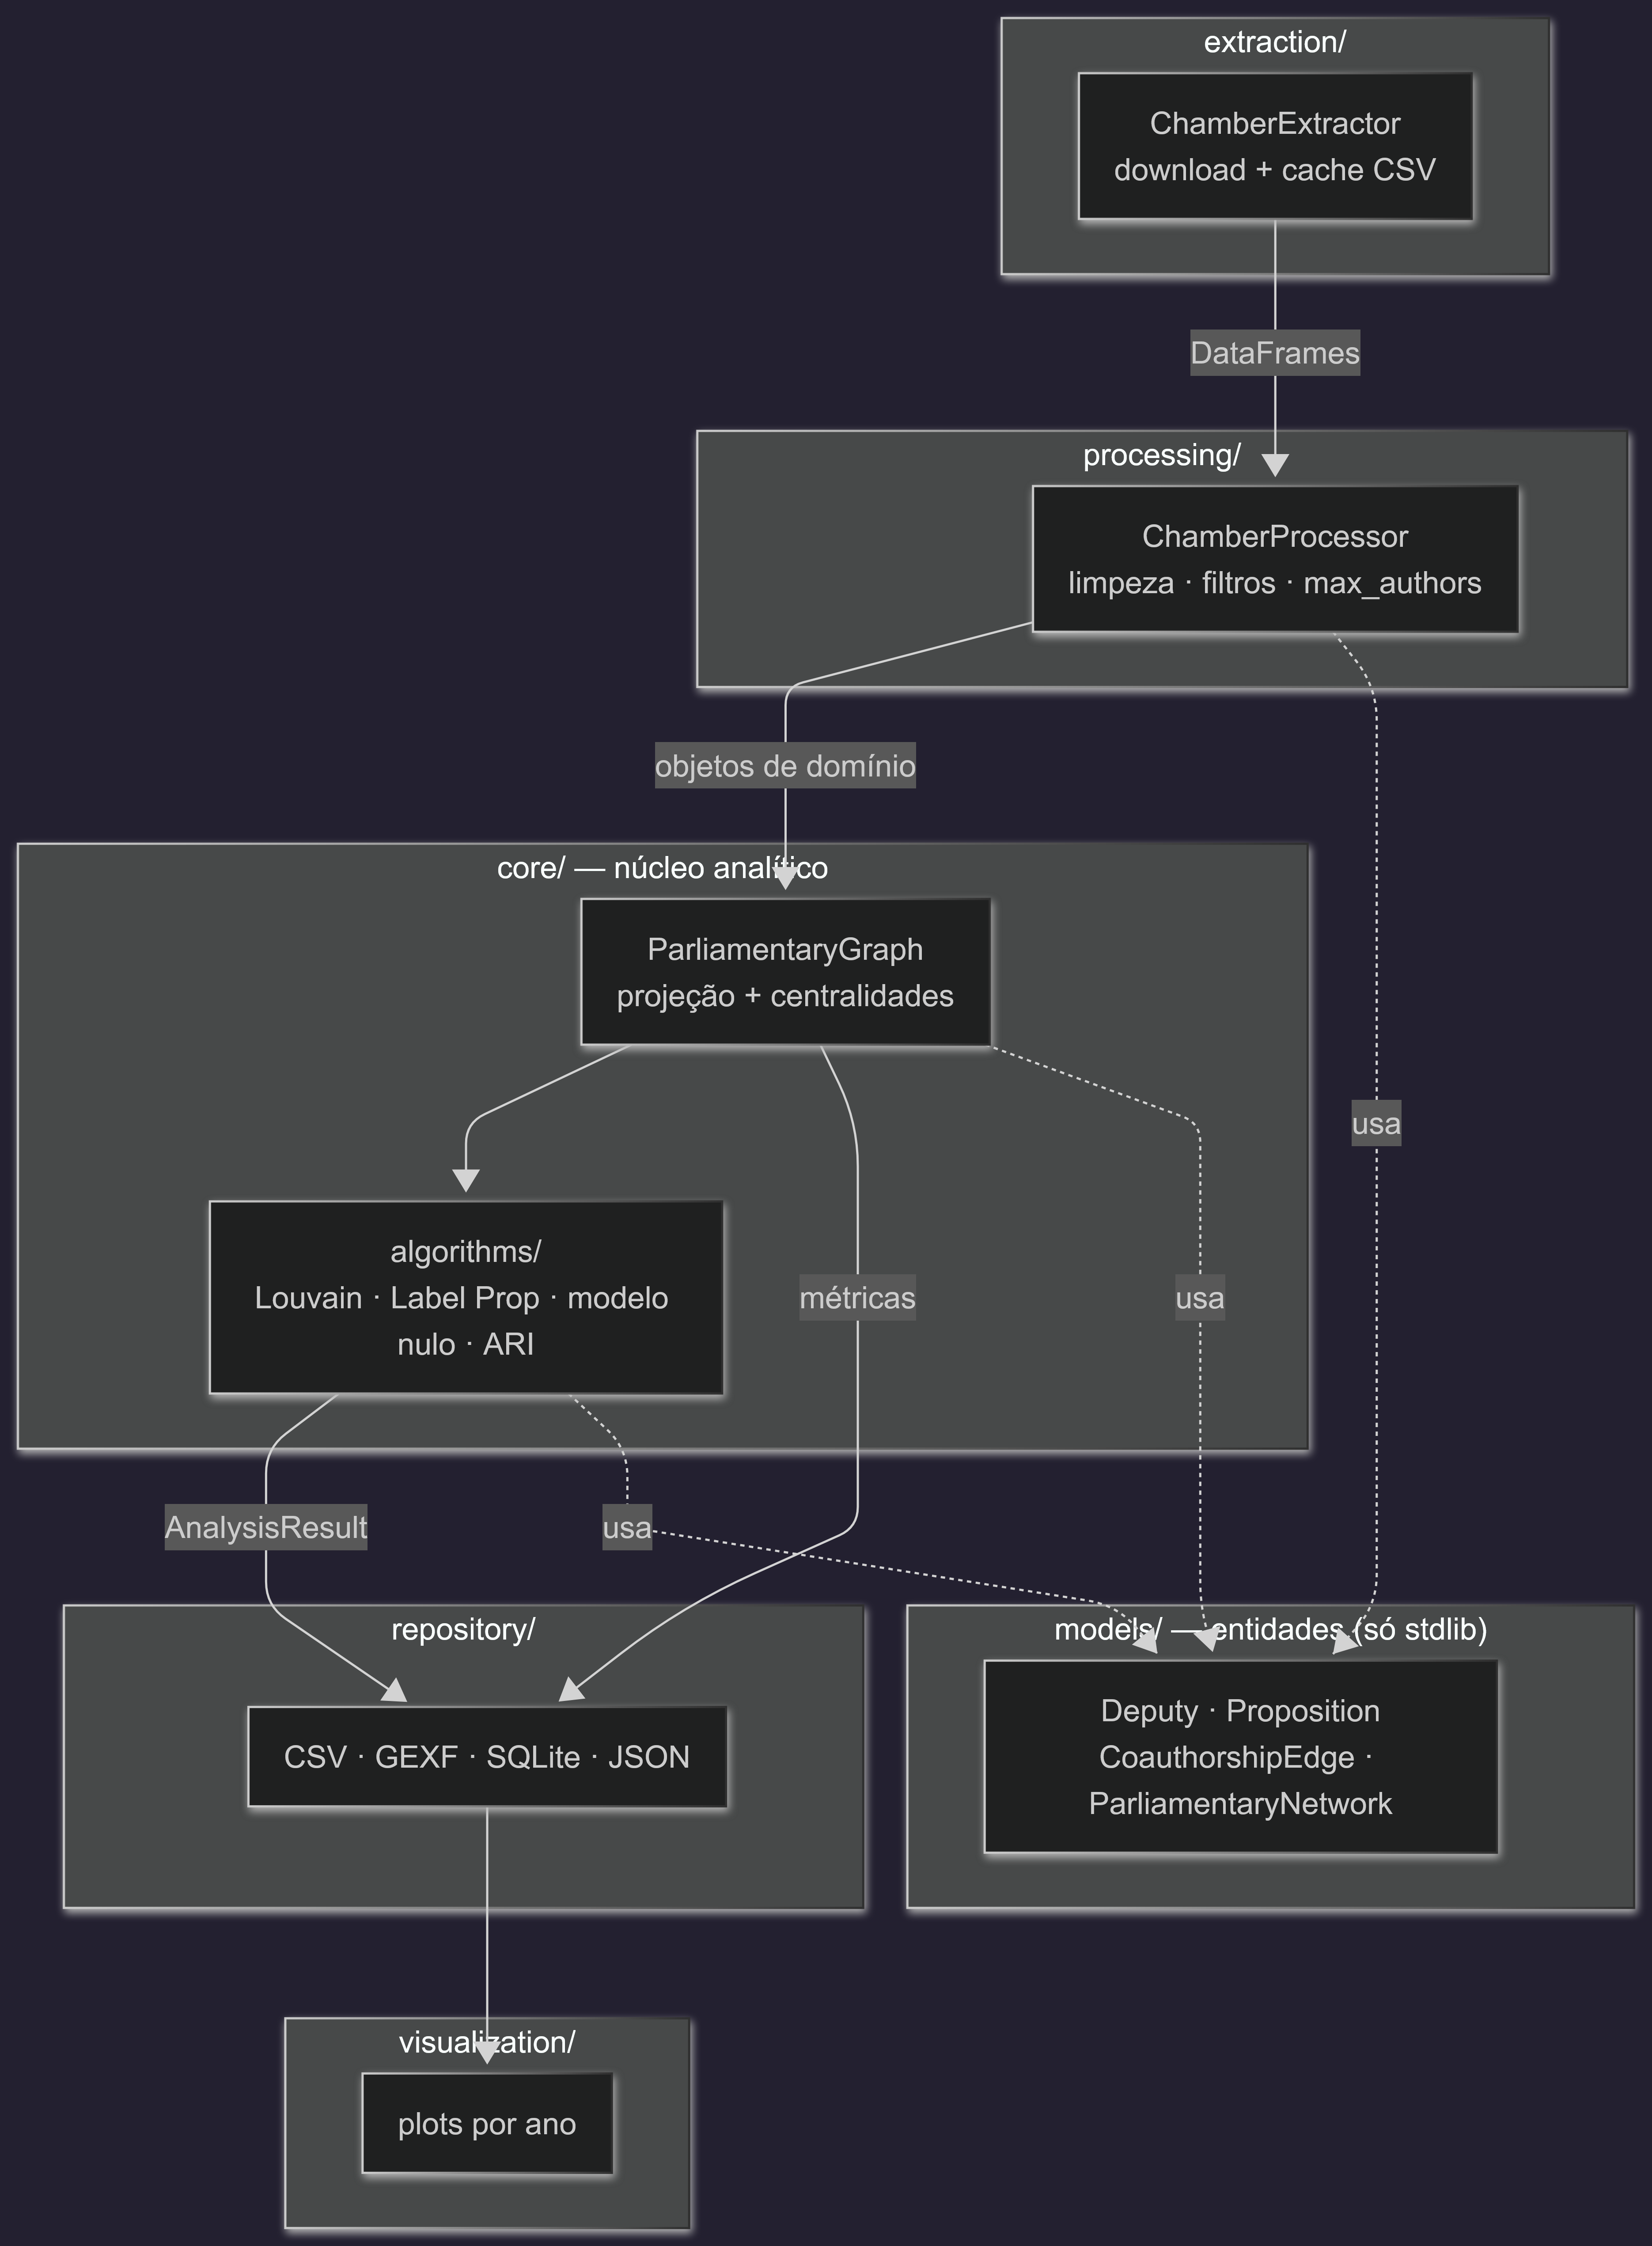
\includegraphics[width=0.6\textwidth]{imagens/componentes.png}
    \fonte{Elaborado pelo autor.}
\end{figure}

A dependência entre camadas respeita a Regra da Dependência da Arquitetura Limpa: camadas inferiores (extraction, repository) dependem das superiores (models, core), nunca o contrário. Cada camada é um pacote Python independente, contido em \texttt{src/}.

\subsection{Models (Entidades)}

A camada \texttt{models/} contém as entidades de domínio puro, implementadas como \textit{dataclasses} do Python (estruturas imutáveis-por-convenção com sintaxe declarativa). Não há dependência de bibliotecas externas além da biblioteca padrão.

\begin{itemize}
    \item \texttt{Deputy}: representa um deputado federal, com identificador único, nome, sigla do partido, sigla da unidade federativa, os cinco campos de métricas de centralidade computadas e a comunidade Louvain atribuída (\texttt{community\_louvain});
    \item \texttt{Proposition}: representa uma proposição legislativa, com identificador, ano, lista de identificadores de autores e tipo (PL, PEC etc.);
    \item \texttt{CoauthorshipEdge}: representa uma aresta da rede de coautoria, com identificadores de origem e destino, peso bruto e peso normalizado;
    \item \texttt{ParliamentaryNetwork}: agregador que contém o grafo NetworkX construído e o dicionário de deputados, fornecendo a interface canônica para as camadas analíticas.
\end{itemize}

\subsection{Core (Casos de Uso)}

A camada \texttt{core/} é o núcleo analítico do sistema, contendo a classe \texttt{ParliamentaryGraph} e os submódulos \texttt{algorithms/}. É a camada de mais alta criticidade --- justificando a cobertura por testes $\geq$ 93\%.

A classe \texttt{ParliamentaryGraph} encapsula:

\begin{itemize}
    \item Construção do grafo a partir das estruturas de coautoria, aplicando a fórmula de ponderação apresentada na Equação~\ref{eq:peso_coautoria};
    \item Cálculo das quatro métricas de centralidade descritas na metodologia;
    \item Atribuição das comunidades detectadas aos objetos \texttt{Deputy} (\texttt{assign\_communities});
    \item Resolução de \textit{aliases} de identificadores (deputados com múltiplos IDs no sistema da Câmara).
\end{itemize}

O submódulo \texttt{algorithms/} agrupa funções puras, isoladas de qualquer preocupação de entrada e saída:

\begin{itemize}
    \item \texttt{metrics.py}: cálculo de centralidades e normalização;
    \item \texttt{community\_detection.py}: implementações encapsuladas dos algoritmos Louvain e Label Propagation, com cálculo de modularidade;
    \item \texttt{validation.py}: teste de permutação contra modelo nulo, que operacionaliza a hipótese central (H1);
    \item \texttt{analysis\_result.py}: \textit{dataclass} agregadora que compõe todos os resultados analíticos de um ano em um objeto tipado, incluindo o cálculo do \textit{Adjusted Rand Index}.
\end{itemize}

\subsection{Extraction e Processing (Adaptadores de Interface)}

A camada \texttt{extraction/} contém a classe \texttt{ChamberExtractor}, responsável pelo download e cache dos CSVs do Portal de Dados Abertos. Implementa: (i) verificação de existência local antes do download, reutilizando o cache quando presente; (ii) download direto dos arquivos CSV do portal via \texttt{pandas}; (iii) persistência do arquivo no diretório de cache local; (iv) reaproveitamento determinístico do cache em execuções subsequentes, tornando a série reprodutível sem depender da rede.

A camada \texttt{processing/} contém a classe \texttt{ChamberProcessor}, responsável por:

\begin{enumerate}
    \item Padronização das colunas (minúsculas, sem espaços);
    \item Filtro de tipos de proposição (PL, PEC, PLP, PDL, EMC);
    \item \textit{Inner join} entre autores e proposições filtradas;
    \item Filtro de domínio (apenas deputados federais, código de tipo de autor 10000);
    \item Construção da estrutura de coautorias, agrupada por proposição;
    \item Aplicação do filtro de massa de signatários (\texttt{max\_authors=30});
    \item Sanitização de valores nulos em sigla de partido e UF (substituídos por sentinelas \texttt{"S/PARTIDO"} e \texttt{"S/UF"});
    \item Conversão das estruturas tabulares em objetos de domínio.
\end{enumerate}

\begin{figure}[H]
    \centering
    \caption{Fluxo de junção e filtragem dos arquivos CSV até a construção
    da rede de coautoria.}
    \label{fig:juncao_dados}
    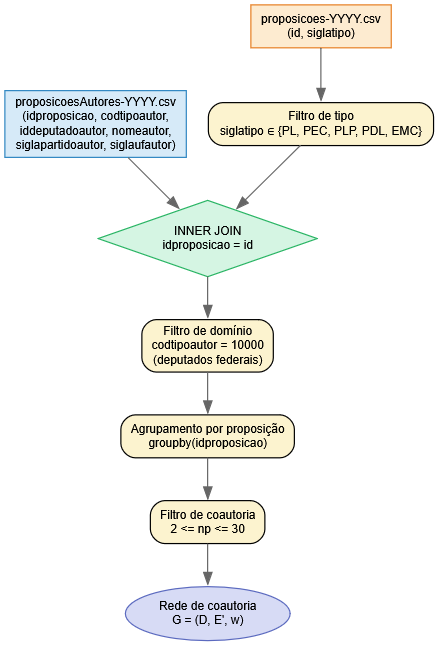
\includegraphics[width=0.6\textwidth]{imagens/juncao_dados.png}
    \fonte{Elaborado pelo autor usando Graphviz Online (2026).}
\end{figure}

A ~\ref{fig:juncao_dados} ilustra as fases das operações. O cruzamento
entre os dois arquivos é realizado por um \textit{inner join} sobre a chave
comum --- o identificador da proposição, nomeado \texttt{idproposicao} no
arquivo de autores e \texttt{id} no de metadados. Essa operação atua como
filtro atômico: ao restringir previamente os metadados aos cinco tipos de
proposição de interesse, o join descarta automaticamente dezenas de milhares
de requerimentos, ofícios e matérias administrativas, sem necessidade de
filtragem posterior. As etapas subsequentes de filtragem por número de
signatários são justificadas na Subseção~\ref{subsec:heuristica}.

\subsection{Repository (Frameworks e Drivers)}

A camada \texttt{repository/} contém quatro adaptadores de persistência:

\begin{itemize}
    \item \texttt{CsvRepository}: exporta métricas de deputados e arestas para arquivos CSV, ordenados por centralidade decrescente, incluindo a coluna de comunidade;
    \item \texttt{GraphExporter}: exporta o grafo NetworkX no formato GEXF, padrão de interoperabilidade com a ferramenta Gephi;
    \item \texttt{DB\_Exporter}: persiste métricas em banco SQLite, com operação \textit{upsert} (insere ou atualiza por chave composta ano $+$ ID) e migração idempotente de esquema via \texttt{ALTER TABLE};
    \item \texttt{AnalysisRepository}: serializa o resultado analítico agregado do ano (\texttt{AnalysisResult}) em arquivo JSON legível e auditável, e o recarrega de forma tipada quando necessário.
\end{itemize}

Adicionalmente, a camada \texttt{visualization/} consome os dados gerados e produz figuras (PNG) e relatório textual (TXT) por ano, organizados em subdiretórios \texttt{data/plots/\{ano\}/}.

\section{MODELAGEM DO GRAFO PARLAMENTAR E HEURÍSTICA DE PONDERAÇÃO}

A construção do grafo segue a fórmula apresentada na Equação~\ref{eq:peso_coautoria}, implementada na classe \texttt{ParliamentaryGraph}. Para cada proposição $p \in P_{\text{filtrado}}$ com $n_p$ coautores:

\begin{enumerate}
    \item Gera-se o conjunto $\{(i, j) : i, j \in \text{autores}(p),\ i < j\}$ de pares ordenados;
    \item Para cada par, adiciona-se $1/(n_p - 1)$ ao peso acumulado da aresta no grafo.
\end{enumerate}

\subsection{Projetos de Lei (PL)}

Os Projetos de Lei são a categoria mais numerosa e diversa de proposições no dataset analisado. Caracterizam-se por ampla variabilidade no número de coautores --- de proposições individuais a iniciativas com dezenas de signatários. Sob a heurística adotada, PLs com poucos coautores contribuem mais fortemente para as arestas, refletindo coordenação política mais específica.

\subsection{Projetos de Lei Complementar (PLP)}

Os Projetos de Lei Complementar, por exigirem maioria absoluta para aprovação e tratarem de matérias constitucionalmente reservadas, tendem a apresentar coautorias mais selecionadas. No dataset analisado, sua presença numérica é menor que a de PLs, mas sua contribuição estrutural à rede é comparativamente densa.

\subsection{Propostas de Emenda à Constituição (PEC)}

PECs são, simultaneamente, os instrumentos legislativos de maior peso simbólico e os principais responsáveis pelo viés de massa de signatários. Por exigirem 171 assinaturas para apresentação (um terço da Câmara), PECs frequentemente acumulam centenas de coautores. A heurística de ponderação $1/(n_p - 1)$ reduz essa influência distorciva, e o filtro \texttt{max\_authors=30} elimina o efeito catastrófico de PECs de massa sobre a topologia da rede.

\section{IMPLEMENTAÇÃO DO NÚCLEO ANALÍTICO COMPUTACIONAL}

Escrever algo...

\subsection{Cálculo de Centralidades}

As centralidades são computadas via funções da biblioteca NetworkX, que implementa internamente algoritmos clássicos:

\begin{itemize}
    \item Grau ponderado: \texttt{graph.degree(weight="weight")};
    \item Intermediação: algoritmo de \cite{brandes2001}, complexidade $O(|V| \cdot |E|)$ em grafos esparsos;
    \item Proximidade: implementação \textit{Dijkstra-based} para grafos ponderados;
    \item Autovetor: método de potência iterativo até convergência.
\end{itemize}

Os valores normalizados são atribuídos aos campos correspondentes do objeto \texttt{Deputy} via método \texttt{compute\_all\_centralities}, mantendo a integridade referencial entre o grafo e a coleção de entidades.

\subsection{Detecção de Comunidades}

A detecção de comunidades é encapsulada na classe \texttt{CommunityDetector}, que expõe três métodos, conforme ilustrado na Listagem~\ref{lst:community}:

\begin{lstlisting}[language=Python, caption={Interface da classe CommunityDetector.}, label={lst:community}]
class CommunityDetector:
    def detect_louvain(self, graph, seed=42) -> dict:
        """Returns {node_id: community_id}"""

    def detect_label_propagation(self, graph) -> dict:
        """Returns {node_id: community_id}"""

    def calculate_modularity(self, graph, partition) -> float:
        """Returns Q value for a given partition"""
\end{lstlisting}

A semente \texttt{seed=42} fixa a sequência pseudo-aleatória interna do Louvain, garantindo que execuções repetidas com o mesmo grafo produzam exatamente a mesma partição --- requisito fundamental para reprodutibilidade científica.

A validação por modelo nulo é implementada em \texttt{algorithms/validation.py}, na função \texttt{assess\_community\_significance}, que executa 200 iterações de \textit{double-edge-swap} (preservando a sequência de graus), recalcula Louvain em cada iteração, e retorna um objeto \texttt{NullModelResult} com as estatísticas agregadas.

\subsection{Persistência dos Resultados Analíticos}

Ao final da etapa analítica de cada ano, todos os resultados --- métricas
topológicas, resumos das partições Louvain e Label Propagation, o \textit{Adjusted
Rand Index} e o resultado do modelo nulo (H1) --- são compostos em um objeto
tipado \texttt{AnalysisResult} e serializados pela \texttt{AnalysisRepository} em
\texttt{data/analysis/analysis\_YYYY.json}. Esse arquivo, além de conter os
metadados de execução (\textit{timestamp}, \texttt{max\_authors},
\texttt{n\_permutations}), é a fonte única de verdade consumida tanto pela
análise comparativa entre anos quanto pela elaboração das tabelas do
Capítulo~\ref{cap:resultados}, eliminando a necessidade de reexecutar o pipeline
para obter qualquer número reportado.

\section{QUALIDADE, INFRAESTRUTURA E REPRODUTIBILIDADE}

escrever algo...

\subsection{Suíte de testes}

O sistema é coberto por 210 testes automatizados, distribuídos em módulos que
cobrem entidades de domínio, construção e análise do grafo, algoritmos de
comunidade, validação estatística por modelo nulo, repositórios de persistência e
integridade dos datasets gerados. Um subconjunto de 64 testes de integridade é
parametrizado por ano e verifica, sobre os arquivos efetivamente produzidos pelo
pipeline, a conformidade de esquema, faixas de valores plausíveis, ausência de
nulos críticos, coerência CSV $\leftrightarrow$ GEXF e plausibilidade estatística
(densidade, modularidade, componente principal).

A cobertura total é de 83\%, com o núcleo analítico (\texttt{core/}) atingindo
$\geq$ 93\% em todos os submódulos. Os testes de integridade de datasets
representam contribuição metodológica relevante: além de validar o código,
validam empiricamente as características dos dados produzidos, capturando
regressões silenciosas que testes unitários não detectariam.

\subsection{Empacotamento Docker}

O ambiente de execução completo é definido em três arquivos:

\begin{itemize}
    \item \texttt{Dockerfile}: imagem base Python 3.11-slim, instalação automática de dependências;
    \item \texttt{docker-compose.yml}: três serviços --- \texttt{pipeline\_chamber} (executa o pipeline completo), \texttt{compare} (executa análise comparativa entre anos), \texttt{tests} (executa a suíte de testes);
    \item \texttt{requirements.txt}: lista de bibliotecas Python com versões fixadas.
\end{itemize}

A execução do pipeline completo para os quatro anos (2022--2025) é desencadeada por um único comando: \texttt{docker compose up pipeline\_chamber}. O tempo médio de execução em hardware de classe \textit{desktop} (Intel i5-14600KF, 32\,GB DDR5) é de 15 a 25 minutos.



\subsection{Orquestração do projeto}

O ambiente pode ser orquestrado totalmente pelo shell \texttt{run.sh}, assim como a execução pode ser feita por esse mesmo shell. Ademais, o comando \texttt{./run.sh help} pode ser de utlidade para saber os comandos especificos do shell.

\subsection{Repositório aberto}

O código-fonte completo, juntamente com a documentação técnica, está disponível em repositório público (\url{https://github.com/felipeevil/parliament-graph-architecture}), em conformidade com os princípios de \textit{Open Science}.

%-------------------------------------------------------------------------------------%
\chapter{Resultados e Discussões}
\label{cap:resultados}

% ═══════════════════════════════════════════════════════════════════════
% NORTE DO CAPÍTULO: apresentar os números gerados pelo artefato (tabelas
% com dados reais) e DISCUTIR o que significam. Ordem: (1) o artefato
% funciona/é reprodutível; (2) como é a rede e quem são os centrais;
% (3) as comunidades e o teste de H1; (4) a estabilidade ao longo dos anos.
% Fonte única dos números: data/analysis/*.json e data/metricas/*.csv.
% ═══════════════════════════════════════════════════════════════════════

Este capítulo apresenta os resultados produzidos pelo artefato para o período 2022--2025 e discute seu significado. Primeiro valida-se a arquitetura e sua reprodutibilidade; em seguida, caracterizam-se a rede e os deputados mais centrais; então testa-se a hipótese central (H1) por meio da detecção de comunidades e do modelo nulo; por fim, avalia-se a estabilidade do padrão ao longo dos quatro anos.

\section{VALIDAÇÃO DA ARQUITETURA E REPRODUTIBILIDADE}

% NORTE: mostrar que o artefato "roda" e é confiável, antes de interpretar dados.
\subsection{Desempenho Computacional}

% NORTE: tempo de execução, hardware, determinismo (seed=42), cobertura de testes.
O \textit{pipeline} completo (quatro anos) executa em [PREENCHER: tempo, ex.\ 15--25] minutos em hardware de classe \textit{desktop} (Intel i5-14600KF, 32\,GB DDR5), de forma determinística: a fixação da semente aleatória (\texttt{seed}=42) garante que execuções repetidas produzam resultados idênticos. A suíte de 210 testes automatizados (cobertura total de 83\%, núcleo $\geq$ 93\%) valida a corretude de cada módulo. [PREENCHER: comentar que a execução via Docker replica o ambiente exatamente.]

\subsection{Geração de Artefatos (Interoperabilidade)}

% NORTE: listar os formatos exportados e por que importam (auditabilidade, Gephi).
Cada execução persiste os resultados em formatos abertos e interoperáveis: CSV (métricas por deputado), GEXF (grafo, compatível com o Gephi), SQLite (persistência consultável) e JSON (\texttt{AnalysisResult} auditável). [PREENCHER: destacar que o GEXF permite validação cruzada independente --- abrir no Gephi e recalcular a modularidade confirma os valores do \textit{pipeline}.]

\section{ANÁLISE DE CENTRALIDADE E INFLUÊNCIA PARLAMENTAR}

\subsection{O Grafo Resultante}

% NORTE: apresentar a Tabela 1 (estrutura da rede) e a Tabela 2 (efeito dos filtros).
A Tabela~\ref{tab:metricas_rede} sintetiza a estrutura da rede em cada ano.

\begin{table}[H]
\centering
\caption{Métricas estruturais da rede de coautoria por ano.}
\label{tab:metricas_rede}
\begin{tabular}{lrrrr}
\toprule
\textbf{Indicador} & \textbf{2022} & \textbf{2023} & \textbf{2024} & \textbf{2025} \\
\midrule
Nós (deputados ativos)       & 273   & 360   & 337   & 331   \\
Arestas (coautorias únicas)  & 3.085 & 5.082 & 4.426 & 5.407 \\
Densidade                    & 8,31\% & 7,86\% & 7,82\% & 9,90\% \\
Modularidade Louvain ($Q$)   & 0,596 & 0,640 & 0,634 & 0,634 \\
Comunidades (Louvain)        & 15    & 12    & 14    & 16    \\
\bottomrule
\end{tabular}
\fonte{Elaborado pelo autor.}
\end{table}

% NORTE: justificar EMPIRICAMENTE os filtros (Tabela do 85%). Argumento forte p/ banca.
A relevância dos filtros de modelagem (Seção~\ref{subsec:heuristica}) é confirmada empiricamente. A Tabela~\ref{tab:filtros} mostra o efeito do filtro de massa de signatários sobre a densidade em 2025.

\begin{table}[H]
\centering
\caption{Efeito do filtro de massa de signatários sobre a densidade (2025).}
\label{tab:filtros}
\begin{tabular}{lrr}
\toprule
\textbf{Configuração} & \textbf{Arestas} & \textbf{Densidade} \\
\midrule
Sem filtro de massa (apenas tipo)      & 124.671 & 85,35\% \\
Com filtro (\texttt{max\_authors}=30)  & 5.407   & 9,90\%  \\
\bottomrule
\end{tabular}
\fonte{Elaborado pelo autor.}
\end{table}

A remoção de 70 proposições com mais de 30 coautores --- a maior com 226 signatários (uma PEC) --- reduz a densidade de 85,35\% para 9,90\%, transformando um grafo quase-completo em uma rede analisável. [PREENCHER: reforçar que a normalização $1/(n_p-1)$ trata a distorção de \emph{peso}, enquanto o filtro trata a distorção \emph{topológica} (existência de arestas) --- os dois são complementares.]

\subsection{Os Deputados mais Influentes}

% NORTE: Tabela dos top-centrais (2025) + a DISCUSSÃO mais importante do trabalho:
% centralidade de coautoria mede ARTICULAÇÃO, não poder institucional.
A Tabela~\ref{tab:top_deputados} apresenta os deputados de maior centralidade em 2025, sob duas óticas: intermediação (pontes entre grupos) e grau ponderado (intensidade de colaboração).

\begin{table}[H]
\centering
\caption{Deputados de maior centralidade em 2025.}
\label{tab:top_deputados}
\begin{tabular}{ll}
\toprule
\textbf{Top intermediação (pontes)} & \textbf{Top grau ponderado (coesão)} \\
\midrule
Franciane Bayer (REPUBLICANOS) & Célia Xakriabá (PSOL)       \\
Alberto Fraga (PL)             & Adriana Ventura (NOVO)       \\
Bibo Nunes (PL)                & Fernanda Melchionna (PSOL)   \\
Pezenti (MDB)                  & Marcel van Hattem (NOVO)     \\
Evair Vieira de Melo (PP)      & Luiz Lima (PL)               \\
\bottomrule
\end{tabular}
\fonte{Elaborado pelo autor.}
\end{table}

% NORTE (parágrafo-chave da defesa): dois achados a discutir.
[PREENCHER: Achado 1 --- as pontes se distribuem por vários partidos (REPUBLIC, PL, MDB, PP), e o principal \textit{broker} não é do maior bloco: o papel de ponte é estrutural e individual, não determinado pelo tamanho do partido.]

[PREENCHER: Achado 2 (o mais importante) --- o grau ponderado é dominado por partidos pequenos e ideologicamente coesos (PSOL, NOVO), que coassinam intensamente em bloco. Isso revela que a centralidade de coautoria mede \textbf{intensidade de articulação}, e \textbf{não poder institucional} (relatorias, presidência de comissões, controle de pauta) --- daí lideranças formais não aparecerem no topo. Retomar aqui a definição operacional de influência da Seção de métodos.]

% NORTE: responde a pergunta norteadora (i) --- concentração da articulação em poucos.
A concentração da articulação em poucos parlamentares --- primeira pergunta norteadora --- é quantificada pelo coeficiente de Gini \cite{gini1921} da distribuição de cada centralidade (0 indica igualdade total; 1, concentração máxima) e pela participação dos dez deputados mais centrais. A Tabela~\ref{tab:concentracao} apresenta os valores de 2025.

\begin{table}[H]
\centering
\caption{Concentração da centralidade em 2025 (coeficiente de Gini e participação dos 10 mais centrais).}
\label{tab:concentracao}
\begin{tabular}{lrr}
\toprule
\textbf{Métrica} & \textbf{Gini} & \textbf{Top-10} \\
\midrule
Autovetor       & 0,951 & 82\% \\
Intermediação   & 0,740 & 26\% \\
Grau ponderado  & 0,566 & 21\% \\
\bottomrule
\end{tabular}
\fonte{Elaborado pelo autor.}
\end{table}

[PREENCHER: discutir que há forte concentração da articulação, \emph{extrema} no autovetor (Gini 0,95: os dez mais concentram 82\%) --- reflexo direto da câmara de eco de bancadas coesas ---, alta na intermediação (0,74) e moderada no grau (0,57). Ressalvar que é concentração da \emph{articulação} (coautoria), não de poder institucional. Observar que o padrão é estável nos quatro anos (Gini do autovetor entre 0,87 e 0,98), e que a divergência entre as métricas confirma que as quatro dimensões de centralidade não são redundantes.]

\section{DETECÇÃO DE COMUNIDADES E TESTE DA HIPÓTESE CENTRAL}

\subsection{Comparação Louvain vs.\ Label Propagation}

% NORTE: Tabela do ARI (4 anos) + discussão honesta sobre ARI moderado.
A concordância entre as duas partições, medida pelo \textit{Adjusted Rand Index} (ARI), é apresentada na Tabela~\ref{tab:ari}.

\begin{table}[H]
\centering
\caption{Concordância entre Louvain e Label Propagation (ARI) por ano.}
\label{tab:ari}
\begin{tabular}{lrrrr}
\toprule
 & \textbf{2022} & \textbf{2023} & \textbf{2024} & \textbf{2025} \\
\midrule
Comunidades (Louvain)          & 15    & 12    & 14    & 16    \\
Comunidades (Label Prop.)      & 19    & 13    & 12    & 10    \\
ARI                            & 0,325 & 0,281 & 0,416 & 0,423 \\
\bottomrule
\end{tabular}
\fonte{Elaborado pelo autor.}
\end{table}

[PREENCHER: discutir que o ARI é moderado (0,28--0,42), mas que os dois algoritmos convergem no \emph{essencial} --- a existência de forte estrutura modular ---, divergindo apenas na granularidade das fronteiras entre comunidades; o Label Propagation é reconhecidamente instável. Enquadrar como verificação de consistência do sinal, não como identidade de partições.]

\subsection{Análise pela Modularidade (Q) --- Teste da Hipótese H1}

% NORTE: Tabela do modelo nulo (o resultado central) + veredito de H1.
% + cruzamento comunidade × partido (a validação de que as comunidades são reais).
A Tabela~\ref{tab:null_model} apresenta o teste de significância da estrutura comunitária contra o modelo nulo ponderado.

\begin{table}[H]
\centering
\caption{Teste de significância da estrutura comunitária (modelo nulo ponderado, 200 permutações).}
\label{tab:null_model}
\begin{tabular}{lrrrr}
\toprule
 & \textbf{2022} & \textbf{2023} & \textbf{2024} & \textbf{2025} \\
\midrule
$Q_{\text{obs}}$                       & 0,596  & 0,640  & 0,634  & 0,634  \\
$Q_{\text{nulo}}$ (média)              & 0,370  & 0,420  & 0,415  & 0,467  \\
$p$-valor                              & <0,005 & <0,005 & <0,005 & <0,005 \\
Significativo ($\alpha=0{,}05$)        & Sim    & Sim    & Sim    & Sim    \\
\bottomrule
\end{tabular}
\fonte{Elaborado pelo autor.}
\end{table}

Em todos os anos, a modularidade observada supera a média do modelo nulo, e \textbf{nenhum dos 200 grafos nulos atinge $Q_{\text{obs}}$} ($p<0{,}005$). \textbf{A hipótese H1 é, portanto, corroborada}: a estrutura de comunidades da rede é não-aleatória. [PREENCHER: enfatizar que o nulo é \emph{ponderado} (pesos reatribuídos), tornando a comparação homogênea; e que H1 é a condição de validade que autoriza interpretar as comunidades como estruturas reais.]

% NORTE: aqui vai o "ouro" --- mostrar que as comunidades correspondem a partidos.
[PREENCHER: inserir a Tabela do cruzamento comunidade $\times$ partido (gerável a partir de \texttt{data/metricas/deputados\_metricas\_2025.csv}, colunas \texttt{community\_louvain} e \texttt{party\_code}) e discutir que as maiores comunidades são dominadas por partidos reais (ex.: uma comunidade $\approx$54\% PL; outra $\approx$59\% PT; outra concentrando o PSOL) --- ou seja, o algoritmo recupera a realidade partidária \emph{sem} jamais receber rótulo ideológico. Esta é a validação qualitativa exigida na metodologia.]

\section{ANÁLISE TEMPORAL (2022--2025)}
\label{sec:temporal}

\subsection{Estabilidade do Padrão Estrutural}

% NORTE: mostrar que Q e o veredito de H1 se mantêm nos 4 anos (persistência).
[PREENCHER: observar que $Q_{\text{obs}}$ permanece na faixa estreita $[0{,}596;\ 0{,}640]$ e que H1 é confirmada em todos os anos --- a fragmentação em comunidades é um padrão \emph{persistente}, não um artefato de um ano específico. Comentar a densidade ligeiramente maior em 2025.]

\subsection{Discussão Longitudinal}

% NORTE: a ressalva metodológica do recorte + leitura política prudente.
[PREENCHER: ressalvar que 2022 pertence à 56ª Legislatura (encerramento, ano eleitoral) enquanto 2023--2025 são da 57ª --- portanto 2022 é ponto de referência de persistência, não comparação ponto-a-ponto homogênea. Discutir, com prudência, o que a estabilidade sugere sobre o comportamento legislativo, sem extrapolar além do que a coautoria (proxy de articulação) permite afirmar.]

%-------------------------------------------------------------------------------------%
\chapter{Conclusão}
\label{cap:conclusao}

% ═══════════════════════════════════════════════════════════════════════
% NORTE DO CAPÍTULO: retomar o problema, afirmar o que foi entregue (o
% artefato) e o que foi demonstrado (H1), listar contribuições, reconhecer
% limitações com honestidade e apontar trabalhos futuros. Manter o fio DSR:
% a contribuição é a ARQUITETURA; a análise é a demonstração de que funciona.
% ═══════════════════════════════════════════════════════════════════════

\section{SÍNTESE DOS ACHADOS}

% NORTE: 1 parágrafo respondendo ao problema de pesquisa.
[PREENCHER: retomar o objetivo geral e afirmar que foi cumprido --- construiu-se e validou-se uma arquitetura reprodutível que transforma dados legislativos brutos em evidências mensuráveis. H1 foi corroborada nos quatro anos ($p<0{,}005$); as centralidades e comunidades caracterizam as estruturas de influência, com o achado de que a coautoria mede articulação (não poder institucional).]

\section{CONTRIBUIÇÕES}

\subsection{Contribuição técnica}

% NORTE: o artefato em si.
[PREENCHER: a arquitetura modular reprodutível (Arquitetura Limpa + SOLID), auditável, containerizada, coberta por 210 testes (incluindo testes de integridade de dataset), independente de reexecução --- ferramenta reutilizável para análises legislativas computacionais.]

\subsection{Contribuição analítica}

% NORTE: o que a aplicação revelou.
[PREENCHER: a caracterização estrutural do legislativo 2022--2025 --- estrutura modular não-aleatória persistente, comunidades que recuperam a organização partidária, e a distinção empírica entre articulação (coautoria) e poder institucional.]

\section{LIMITAÇÕES}

% NORTE: seção que IMPRESSIONA a banca. Ser honesto = força, não fraqueza.
[PREENCHER, em itens:]
\begin{itemize}
    \item \textbf{Coautoria como \textit{proxy}}: mede articulação, não voto igual nem posição ideológica formal; dois adversários podem coassinar um projeto pontual.
    \item \textbf{Centralidade $\neq$ poder institucional}: a rede não captura relatorias, presidência de comissões ou controle de pauta.
    \item \textbf{ARI moderado} (0,28--0,42): os algoritmos divergem na granularidade das fronteiras.
    \item \textbf{Recorte de 2022}: pertence à 56ª Legislatura (ano eleitoral atípico).
    \item \textbf{Parâmetro \texttt{max\_authors}=30}: escolha conservadora; análise de sensibilidade fica como trabalho futuro. [PREENCHER: se já tiver rodado 20/30/40, mover para os resultados.]
    \item \textbf{Acoplamento à fonte}: o artefato depende do esquema de CSV da Câmara.
\end{itemize}

\section{TRABALHOS FUTUROS}

% NORTE: caminhos concretos (vários já estão nos slides).
\begin{itemize}
    \item Análise de sensibilidade dos parâmetros (\texttt{max\_authors}, filtro de tipos).
    \item Comparação com o algoritmo de Leiden \citeonline{traag2019}.
    \item Cruzamento com dados de votação nominal, testando se a coautoria prediz votos.
    \item Extensão da série histórica e aprofundamento da análise longitudinal.
    \item Aplicação de Redes Neurais de Grafos (GNNs) para predição de comportamento legislativo.
\end{itemize}

\section{CONSIDERAÇÕES FINAIS}

% NORTE: fechamento curto, retomando o valor do artefato (transparência/auditoria).
[PREENCHER: parágrafo final --- reforçar o valor de uma ferramenta aberta e auditável para transparência parlamentar, unindo engenharia de software e método científico, e convidar à reutilização/extensão do artefato.]

%-------------------------------------------------------------------------------------%
%                             P Ó S   T E X T U A L                                  %
%-------------------------------------------------------------------------------------%
    \postextual

%-------------------------------------------------------------------------------------%
% R E F E R Ê N C I A S
%-------------------------------------------------------------------------------------%
    \bibliography{referencias}

%-------------------------------------------------------------------------------------%
% A P Ê N D I C E S
%-------------------------------------------------------------------------------------%
    \begin{apendicesenv}

        \chapter{ESTRUTURA DO REPOSITÓRIO DE CÓDIGO}

        O código-fonte completo do artefato desenvolvido neste trabalho está
        disponível publicamente em
        \url{https://github.com/felipeevil/parliament-graph-architecture}. O
        repositório segue a seguinte estrutura modular:

        \begin{itemize}
            \item \texttt{src/config/}: configuração centralizada (variáveis de ambiente, constantes, logger);
            \item \texttt{src/core/}: núcleo analítico (classe \texttt{ParliamentaryGraph} e submódulo \texttt{algorithms/});
            \item \texttt{src/extraction/}: camada de extração (\texttt{ChamberExtractor});
            \item \texttt{src/models/}: entidades de domínio (\texttt{Deputy}, \texttt{Proposition}, \texttt{CoauthorshipEdge});
            \item \texttt{src/processing/}: limpeza, filtros e conversão para objetos de domínio (\texttt{ChamberProcessor});
            \item \texttt{src/repository/}: persistência (CSV, GEXF, SQLite, JSON);
            \item \texttt{src/visualization/}: geração automática de figuras;
            \item \texttt{src/tests/}: suíte de testes (210 testes);
            \item \texttt{scripts/}: utilitários auxiliares (análise comparativa entre anos);
            \item \texttt{data/}: artefatos gerados em tempo de execução (não versionados);
            \item \texttt{Dockerfile}, \texttt{docker-compose.yml}, \texttt{requirements.txt}: empacotamento reprodutível.
        \end{itemize}

    \end{apendicesenv}

%-------------------------------------------------------------------------------------%
% A N E X O S
%-------------------------------------------------------------------------------------%
    % \begin{anexosenv}
    %     \chapter{TÍTULO DO ANEXO}
    %     % \includepdf[pages=-]{nome_do_arquivo.pdf}
    % \end{anexosenv}

\end{document}